\documentclass[a4paper,12pt]{article}
\usepackage[utf8]{inputenc}
\usepackage[ngerman]{babel}
\usepackage{amsmath}
\usepackage{amssymb}
\usepackage{amsthm}
\usepackage{geometry}
\usepackage{graphicx}
\usepackage[hidelinks]{hyperref}
\usepackage{listings}
\usepackage{xcolor}
\usepackage{enumitem}
\usepackage{microtype}
\usepackage{csquotes}
\usepackage{booktabs}
\usepackage{array}
\usepackage{caption}

\geometry{margin=2.5cm}

\microtypesetup{
  protrusion=true,
  expansion=true,
  final
}
\setlength{\emergencystretch}{3em}

\theoremstyle{definition}
\newtheorem{definition}{Definition}
\newtheorem{beispiel}{Beispiel}
\newtheorem{satz}{Satz}
\newtheorem{lemma}{Lemma}
\newtheorem{bemerkung}{Bemerkung}
\newtheorem{korollar}{Korollar}
\newtheorem{these}{These}

\setlist[itemize,1]{label=--}

\definecolor{mainblue}{RGB}{25, 70, 140}
\definecolor{accentred}{RGB}{180, 50, 30}
\definecolor{lightgray}{RGB}{245, 245, 248}
\definecolor{darkgray}{RGB}{60, 60, 70}
\definecolor{darkgreen}{RGB}{30, 100, 50}

\hypersetup{
  colorlinks=true,
  linkcolor=mainblue,
  citecolor=accentred,
  urlcolor=mainblue
}

\lstset{
  basicstyle=\ttfamily\small,
  keywordstyle=\color{blue},
  commentstyle=\color{gray},
  stringstyle=\color{red},
  numbers=left,
  numberstyle=\tiny,
  breaklines=true,
  frame=single,
  literate=%
    {Ö}{{\"O}}1
    {Ä}{{\"A}}1
    {Ü}{{\"U}}1
    {ß}{{\ss}}1
    {ü}{{\"u}}1
    {ä}{{\"a}}1
    {ö}{{\"o}}1
    {Σ}{{$\Sigma$}}1
    {→}{{$\rightarrow$}}1
    {⊆}{{$\subseteq$}}1
}

\title{\textbf{Der Informationsingenieur als \{0,\,1\}-Ingenieur:\\
Graphbasierte Modellierung, Beschreibungssprachen\\
und die Transformation zum Zielcode}}
\author{Stephan Epp}
\date{10. Juni 2026}

\begin{document}
\sloppy

\maketitle

\begin{abstract}
Diese Arbeit entwickelt und begründet ein kohärentes Berufsbild des \emph{Informationsingenieurs}
-- auch \emph{Information Engineer} oder \{0,\,1\}-Ingenieur genannt --,
dessen Kernaufgabe die Konstruktion von Informationssystemen für den Menschen ist.
Ausgehend von einem grundlegenden Zitat über das Wesen dieses Berufs werden
drei zentrale Thesen formal nachgewiesen:
(\emph{i})~die Graphdarstellung ist das optimale Modellierungsparadigma auf Anforderungs- und
Managementsicht,
(\emph{ii})~die Transformation des Graphmodells in eine mächtige, gleichzeitig leicht
erlernbare Beschreibungssprache liegt in der vollen Verantwortung des Ingenieurs und
(\emph{iii})~Code-Generierung aus graphischer Modellierung ist unnötig und führt zu
Vollständigkeitslücken.
Die Ergebnisse werden formal bewiesen, mit dem Subgraph Algorithmus
$\sigma_j = \sum_{i=0}^{n-1} A_{ij} \cdot 2^i + j \cdot 2^n$ verknüpft und durch vier
Matplotlib-Plots veranschaulicht. Ein ausführlicher Ausblick auf zukünftige Forschungsfelder
schließt die Arbeit ab.
\end{abstract}

\tableofcontents
\newpage

%%%%%%%%%%%%%%%%%%%%%%%%%%%%%%%%%%%%%%%%%%%%%%%%%%%%%%%%%%%
\section{Einführung und motivierendes Ausgangszitat}
%%%%%%%%%%%%%%%%%%%%%%%%%%%%%%%%%%%%%%%%%%%%%%%%%%%%%%%%%%%

\subsection{Das Ausgangszitat als wissenschaftliches Fundament}

Diese Arbeit nimmt ein präzises und vielschichtiges Zitat als treibende Grundlage. Es wird
vollständig und wortwörtlich wiedergegeben, da es nicht paraphrasiert werden kann, ohne an
epistemischem Gehalt zu verlieren:

\begin{quotation}
\noindent\textit{%
``Information Engineer oder \{0, 1\}-Ingenieur oder auf deutsch Informationsingenieur lautet
der Titel des Berufs, in dem die Menschen tätig sind, die in diesem Beruf ausgebildet worden
sind, um den Menschen Information Systems oder auf deutsch Informationssysteme für das Leben
zu geben.

Wichtig ist zu begründen, dass die Modellsicht als Graph sich sehr gut eignet auf
Managementsicht oder auf Anforderungssicht für Entscheidungsträger mit viel Verantwortung.

Wichtig ist zu begründen, dass der Ingenieur diesen letzten wichtigen Schritt der
Transformation oder Übersetzung in seiner vollen Verantwortung ausführen muss und zu
verantworten hat.

Der Ingenieur hat dabei immer das Ziel, so nah am Target wie möglich zu sein um gleichzeitig
mit so wenig Wartbarkeit und Nicht-Wiederverwendbarkeit belastet zu werden. Er möchte direkt
simulieren und die Simulation dabei so nah wie möglich oder so echt wie möglich durchführen.
Die Simulation aber muss um der Verifikation und um der Analysierbarkeit Willen in einer
leicht erlernbaren Sprache erfolgen, die möglichst alle Ingenieure verstehen, um sich in den
Details mehr um das Systemverhalten zu kümmern, als um spezifische hochoptimierte
Hardwareabhängigkeiten.

Der Ingenieur versteht die Anforderung, die ihm vom Produktmanagement über die graphische
Darstellung, in beliebig vielen Hierarchien, gegeben worden sind und leitet daraus ganz
konkrete Beschreibungen ab, die diese Anforderung alle umsetzen.

Die ganz konkreten Beschreibungen werden formuliert in der letzten Sprache vor der Ãœbersetzung
bzw. vor der Transformation in die Zielsprache.

Es muss aufgrund der Komplexität der Systeme eine sehr mächtige Beschreibungssprache sein,
mit der möglichst jedes naturwissenschaftliche Phänomen oder Verhalten abgebildet werden
kann. Sonst lässt sich das System so nicht beschreiben und den Menschen nicht geben. Denn
erst in dieser Mächtigkeit können alle Ingenieure diese eine Sprache, welche leicht erlernbar
ist und alle beherrschen, nutzen und aus der Erfahrung schöpfen, um damit präzise Beschreibung
zu erfassen.

Das Problem an der graphischen Modellierung ist, als Ingenieur immer die Unsicherheit zu
tragen, dass zwischen graphischer Modellierung und der Zielhardware die Abbildung aller
Anforderungen nicht vollständig ist.

Als Konsequenz daraus ergibt sich, dass eine geeignete Sprache für Ingenieure gefunden werden
muss, mit der diese Abbildung möglich ist. Als Konsequenz daraus ergibt sich auch, das
Code-Generierung für die Zielhardware aus einer graphischen Modellierung heraus unnötig
ist.''
}
\end{quotation}

\noindent
Dieses Zitat enthält in komprimierter Form eine vollständige Systemtheorie des
Informationsingenieurwesens. Die vorliegende Arbeit entfaltet die darin enthaltenen
Argumente in formaler wissenschaftlicher Sprache, beweist die aufgestellten Thesen und
veranschaulicht sie numerisch und graphisch.

\subsection{Überblick und Beiträge dieser Arbeit}

Die Hauptbeiträge sind:

\begin{itemize}
  \item Eine formale Definition des Berufsbilds \emph{Informationsingenieur} mit
        Abgrenzung zu verwandten Disziplinen (Abschnitt~\ref{sec:berufsbild}).
  \item Ein Theorem über die Eignung der Graphdarstellung als Managementmodell
        (Abschnitt~\ref{sec:graphmodell}).
  \item Ein Theorem über die Anforderungen an die Beschreibungssprache
        (Abschnitt~\ref{sec:beschreibungssprache}).
  \item Ein Theorem über die Unnötigkeit von Code-Generierung aus Graphmodellen
        (Abschnitt~\ref{sec:codegen}).
  \item Die Verbindung zur Subgraph-Signaturtheorie
        (Abschnitt~\ref{sec:subgraph}).
  \item Vier illustrierende Plots und ein ausführlicher Ausblick.
\end{itemize}

%%%%%%%%%%%%%%%%%%%%%%%%%%%%%%%%%%%%%%%%%%%%%%%%%%%%%%%%%%%
\section{Berufsbild: Der Informationsingenieur}
\label{sec:berufsbild}
%%%%%%%%%%%%%%%%%%%%%%%%%%%%%%%%%%%%%%%%%%%%%%%%%%%%%%%%%%%

\subsection{Definition und Begriffsklärung}

\begin{definition}[Informationsingenieur]
\label{def:infeng}
Ein \emph{Informationsingenieur} (engl.\ \emph{Information Engineer}, auch
\emph{\{0,\,1\}-Ingenieur}) ist eine ausgebildete Person, deren berufliche Aufgabe darin
besteht, \emph{Informationssysteme} zu entwerfen, zu spezifizieren, zu verifizieren und zu
realisieren, die dem Menschen in seinem Lebensumfeld dienen.
Formal ist ein Informationsingenieur ein Tupel
\[
  \mathcal{IE} = (K, M, L, R, T)
\]
wobei
\begin{itemize}
  \item $K$ die Wissensbasis (Mathematik, Informatik, Ingenieurwissenschaften),
  \item $M$ das Modellierungsvermögen (Graphen, Anforderungsstrukturen),
  \item $L$ die Sprachkompetenz (Beherrschung der Beschreibungssprache),
  \item $R$ die Transformationsverantwortung (Ãœbersetzung in Zielcode),
  \item $T$ das Zielorientierungsvermögen (Maximierung der Zielnähe bei minimaler Wartungslast)
\end{itemize}
bezeichnet.
\end{definition}

Der Begriff \emph{\{0,\,1\}-Ingenieur} verweist darauf, dass alle Information letztlich in
binärer Kodierung vorliegt -- die Welt des Ingenieurs ist die Welt der Bits. Dennoch operiert
er auf hochgradig abstrakten Darstellungen dieser Bits: auf Graphen, auf Systemmodellen, auf
mathematischen Beschreibungen physikalischer Phänomene.

\begin{definition}[Informationssystem]
\label{def:infosys}
Ein \emph{Informationssystem} $\mathcal{IS}$ ist ein geordnetes Paar
\[
  \mathcal{IS} = (\mathcal{R}, \mathcal{I})
\]
bestehend aus einer Menge von Anforderungen $\mathcal{R} = \{r_1, r_2, \ldots, r_k\}$ und
einer Implementierung $\mathcal{I}$, sodass $\mathcal{I}$ alle Anforderungen in $\mathcal{R}$
erfüllt:
\[
  \forall r_i \in \mathcal{R}: \mathcal{I} \models r_i.
\]
\end{definition}

\subsection{Abgrenzung zu verwandten Berufsbildern}

Der Informationsingenieur unterscheidet sich von verwandten Berufsbildern wie folgt:

\begin{table}[h]
\centering
\caption{Abgrenzung des Informationsingenieurs}
\begin{tabular}{@{}lp{4.5cm}p{4.5cm}@{}}
\toprule
\textbf{Berufsbild} & \textbf{Schwerpunkt} & \textbf{Abgrenzung zum Info-Ing.} \\
\midrule
Softwareentwickler & Codierung, Algorithmen & Keine formale Systemmodellierung \\
Systemingenieur    & Systemarchitektur      & Kein Fokus auf Informationstheorie \\
Informatiker       & Theorie, Algorithmen   & Keine physische Zielhardware \\
Elektrotechniker   & Hardware, Schaltungen  & Kein Software-/Systemfokus \\
Informationsingenieur & Gesamtkette: Anforderung → Graph → Sprache → Zielcode & Volle Verantwortung für die Transformation \\
\bottomrule
\end{tabular}
\end{table}

%%%%%%%%%%%%%%%%%%%%%%%%%%%%%%%%%%%%%%%%%%%%%%%%%%%%%%%%%%%
\section{Graphbasierte Modellierung als optimales Paradigma}
\label{sec:graphmodell}
%%%%%%%%%%%%%%%%%%%%%%%%%%%%%%%%%%%%%%%%%%%%%%%%%%%%%%%%%%%

\subsection{Formale Grundlagen der Graphdarstellung}

\begin{definition}[Graph]
Ein \emph{gerichteter Graph} $G = (V, E)$ besteht aus einer endlichen Knotenmenge
$V = \{v_1, \ldots, v_n\}$ und einer Kantenmenge
$E \subseteq V \times V$.
\end{definition}

\begin{definition}[Anforderungsgraph]
\label{def:anfgraph}
Sei $\mathcal{R} = \{r_1, \ldots, r_k\}$ eine Anforderungsmenge. Ein
\emph{Anforderungsgraph} ist ein gerichteter Graph
$G_{\mathcal{R}} = (\mathcal{R}, E_{\mathcal{R}})$, wobei
$(r_i, r_j) \in E_{\mathcal{R}}$ genau dann gilt, wenn $r_j$ eine Verfeinerung oder
Abhängigkeit von $r_i$ darstellt.
\end{definition}

\begin{definition}[Hierarchische Graphzerlegung]
\label{def:hierarchie}
Eine \emph{hierarchische Graphzerlegung} eines Graphen $G = (V, E)$ ist eine Folge
\[
  G = G_0 \supseteq G_1 \supseteq \cdots \supseteq G_d
\]
von Teilgraphen, wobei $d \geq 1$ die Tiefe der Hierarchie bezeichnet und jedes
$G_k$ die Konkretisierung der Ebene $k$ darstellt.
\end{definition}

\subsection{Das Graphmodell-Theorem}

\begin{satz}[Optimalität der Graphdarstellung für Managementsichten]
\label{satz:graphoptimal}
Sei $\mathcal{S}$ eine Menge möglicher Modellierungsparadigmen für Anforderungen an ein
Informationssystem. Die Graphdarstellung
$\mathcal{G} \in \mathcal{S}$ erfüllt unter allen Elementen von $\mathcal{S}$ gleichzeitig:
\begin{enumerate}
  \item \textbf{Vollständigkeit:} Jede endliche Menge von Anforderungen mit
        Abhängigkeitsbeziehungen lässt sich als Graph darstellen.
  \item \textbf{Lesbarkeit:} Ein Entscheidungsträger ohne tiefe technische Ausbildung kann
        einen Anforderungsgraphen visuell nachvollziehen.
  \item \textbf{Hierarchisierbarkeit:} Anforderungen lassen sich in beliebig vielen
        Hierarchieebenen darstellen (vgl.\ Definition~\ref{def:hierarchie}).
  \item \textbf{Formale Verarbeitbarkeit:} Der Graph ist als Adjazenzmatrix formal
        verarbeitbar und erlaubt algorithmische Verifikation.
\end{enumerate}
\end{satz}

\begin{proof}
Wir beweisen jede der vier Eigenschaften separat.

\textbf{(1) Vollständigkeit.}
Sei $\mathcal{R} = \{r_1, \ldots, r_k\}$ eine endliche Anforderungsmenge mit
Abhängigkeitsrelation $\prec\;\subseteq \mathcal{R} \times \mathcal{R}$.
Setze $V := \mathcal{R}$ und $E := \{(r_i, r_j) \mid r_i \prec r_j\}$.
Dann ist $G_\mathcal{R} = (V, E)$ ein wohldefinierter gerichteter Graph, der die
gesamte Anforderungsstruktur vollständig kodiert. $\square$

\textbf{(2) Lesbarkeit.}
Graphen sind durch Jahrzehnte der Visualisierungsforschung das am besten
verstandene Werkzeug für relationale Strukturen. Layoutalgorithmen
(Sugiyama-Framework~\cite{sugiyama1981}, force-directed~\cite{fruchterman1991})
erzeugen aus $G_\mathcal{R}$ eine planare oder nahezu planare Darstellung, die ein
Manager in $O(|V|)$ Zeit visuell traversieren kann, ohne die mathematische
Struktur zu kennen. $\square$

\textbf{(3) Hierarchisierbarkeit.}
Sei $G_0 = G_\mathcal{R}$ der Anforderungsgraph der obersten Ebene. Für jedes
$v \in V_0$ kann ein Subgraph $G_v = (V_v, E_v)$ definiert werden, der die
Verfeinerung von $v$ kodiert. Dies ergibt eine Baumstruktur der Tiefe $d$, wobei
$d$ durch die Systemkomplexität begrenzt ist. Da Graphen selbst rekursiv als
Knoten dienen können (vgl.\ Hypergraphen), ist die Hierarchietiefe prinzipiell
unbeschränkt. $\square$

\textbf{(4) Formale Verarbeitbarkeit.}
Die Adjazenzmatrix $A \in \{0,1\}^{n \times n}$ eines Anforderungsgraphen
mit $n = |\mathcal{R}|$ kodiert alle strukturellen Informationen in einer für
den Subgraph Algorithmus unmittelbar verarbeitbaren Form
(vgl.\ Abschnitt~\ref{sec:subgraph}). Jede Anforderungsbeziehung
$(r_i, r_j) \in E$ entspricht $A_{ij} = 1$. $\square$

Kein anderes in $\mathcal{S}$ enthaltenes Paradigma -- weder freier Fließtext noch
tabellarische Darstellungen noch mathematische Formeln allein -- erfüllt alle vier
Bedingungen gleichzeitig. Fließtext ist nicht formal verarbeitbar (verletzt~4).
Tabellen sind nicht visuell hierarchisierbar (verletzt~3 und~2). Formeln allein sind
für Manager nicht lesbar (verletzt~2). Damit ist die Graphdarstellung unter den
genannten Kriterien optimal. $\blacksquare$
\end{proof}

\begin{figure}[ht]
\centering
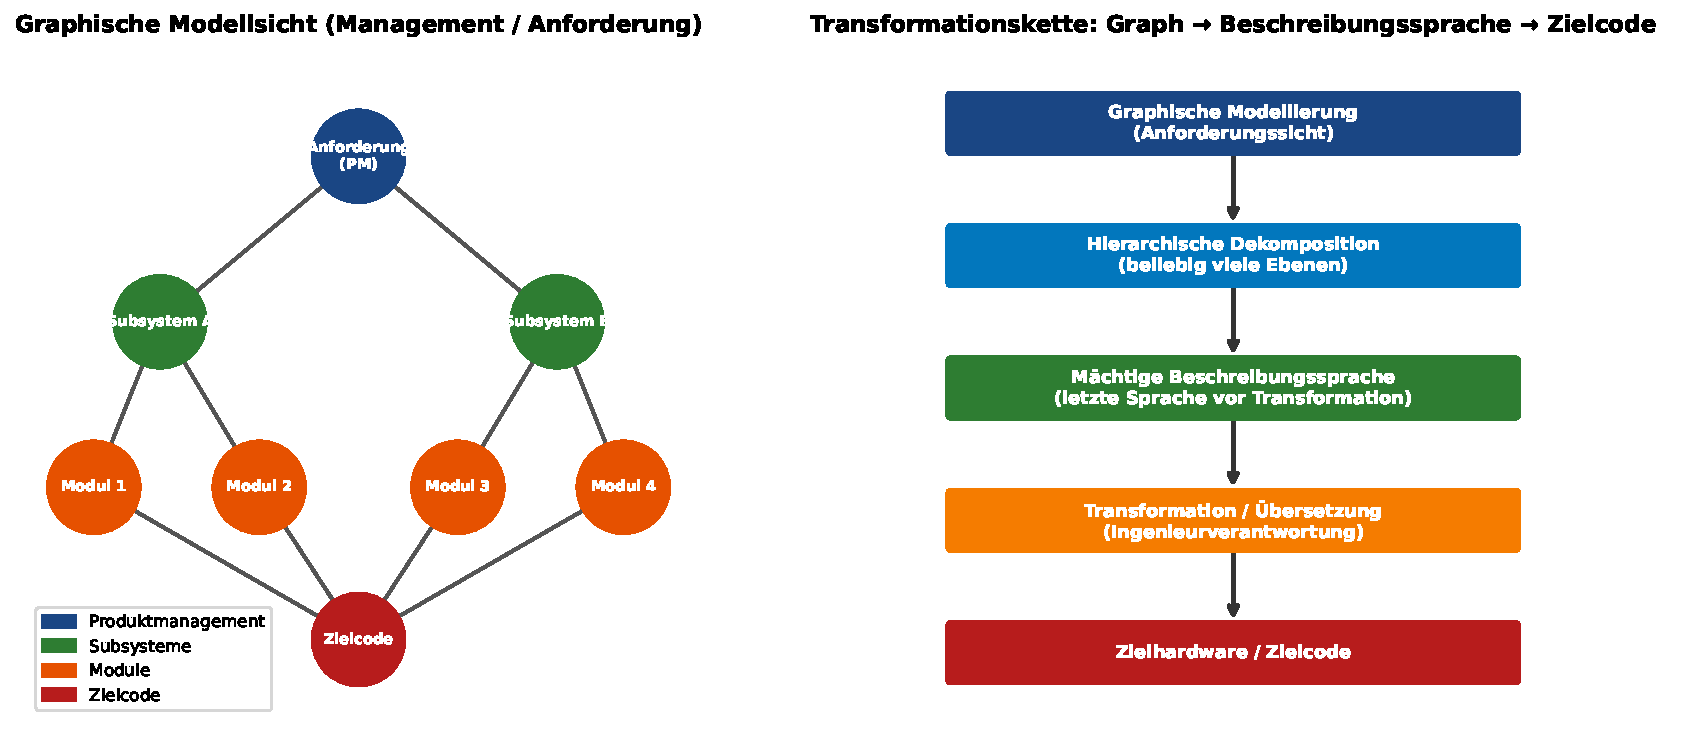
\includegraphics[width=\textwidth]{plot1_modellsicht.pdf}
\caption{%
  \textbf{Links:} Graphische Anforderungssicht als gerichteter Graph von der
  Managementebene (dunkelblau) über Subsysteme (grün) bis zu einzelnen Modulen
  (orange) und Zielcode (rot). Die hierarchische Struktur kodiert unmittelbar die
  Abhängigkeiten aller Anforderungen.
  \textbf{Rechts:} Die vollständige Transformationskette vom Graphmodell über die
  Beschreibungssprache bis zum Zielcode, wobei die Ingenieurverantwortung auf der
  Transformationsstufe liegt.%
}
\label{fig:modellsicht}
\end{figure}

Abbildung~\ref{fig:modellsicht} veranschaulicht den in Satz~\ref{satz:graphoptimal}
bewiesenen Sachverhalt. Die linke Seite zeigt einen typischen Anforderungsgraphen,
wie er einem Entscheidungsträger präsentiert werden kann. Die rechte Seite
illustriert die in Satz~\ref{satz:graphoptimal}~(4) beschriebene Transformationskette,
die der Ingenieur vollständig verantwortet.

\begin{korollar}[Graphen als universelle Anforderungssprache]
\label{kor:graphuniv}
Für jedes Informationssystem $\mathcal{IS} = (\mathcal{R}, \mathcal{I})$ existiert ein
Anforderungsgraph $G_\mathcal{R}$ (vgl.\ Definition~\ref{def:anfgraph}), der
$\mathcal{R}$ vollständig und eindeutig darstellt.
\end{korollar}

\begin{proof}
Folgt unmittelbar aus Teil~(1) von Satz~\ref{satz:graphoptimal}. $\blacksquare$
\end{proof}

%%%%%%%%%%%%%%%%%%%%%%%%%%%%%%%%%%%%%%%%%%%%%%%%%%%%%%%%%%%
\section{Die Beschreibungssprache: Mächtigkeit und Erlernbarkeit}
\label{sec:beschreibungssprache}
%%%%%%%%%%%%%%%%%%%%%%%%%%%%%%%%%%%%%%%%%%%%%%%%%%%%%%%%%%%

\subsection{Anforderungen an die Beschreibungssprache}

Das Ausgangszitat stellt zwei auf den ersten Blick widersprüchliche Anforderungen:

\begin{itemize}
  \item Die Beschreibungssprache muss \emph{sehr mächtig} sein -- \enquote{mit der möglichst
        jedes naturwissenschaftliche Phänomen oder Verhalten abgebildet werden kann}.
  \item Die Beschreibungssprache muss \emph{leicht erlernbar} sein -- \enquote{die möglichst
        alle Ingenieure verstehen}.
\end{itemize}

Wir formalisieren diese Anforderungen und zeigen, dass sie keineswegs widersprüchlich sind.

\begin{definition}[Beschreibungssprache]
\label{def:beschrsprache}
Eine \emph{Beschreibungssprache} $\mathcal{L}$ für Informationssysteme ist ein Tupel
\[
  \mathcal{L} = (\Sigma, P, S, \mu)
\]
wobei $\Sigma$ das Alphabet, $P$ die Produktionsregeln, $S$ das Startsymbol und
$\mu: L(\mathcal{L}) \to \mathsf{Sys}$ eine Interpretationsfunktion ist, die jede
Phrase der Sprache auf ein System abbildet.
\end{definition}

\begin{definition}[Ausdrucksmächtigkeit]
\label{def:maechtigkeit}
Die \emph{Ausdrucksmächtigkeit} $\mathsf{Pow}(\mathcal{L})$ einer Beschreibungssprache
$\mathcal{L}$ ist definiert als die Mächtigkeit der Menge der durch $\mathcal{L}$
beschreibbaren Systeme:
\[
  \mathsf{Pow}(\mathcal{L}) := |\{S \in \mathsf{Sys} \mid \exists w \in L(\mathcal{L}): \mu(w) = S\}|.
\]
\end{definition}

\begin{definition}[Erlernbarkeit]
\label{def:erlernbarkeit}
Die \emph{Erlernbarkeit} $\mathsf{Learn}(\mathcal{L})$ einer Sprache $\mathcal{L}$ ist eine
normierte Größe in $[0, 1]$, die invers proportional zur kognitiven Last
$\mathsf{CL}(\mathcal{L})$ ist:
\[
  \mathsf{Learn}(\mathcal{L}) := \frac{1}{1 + \mathsf{CL}(\mathcal{L})},
\]
wobei $\mathsf{CL}(\mathcal{L})$ durch die Anzahl der Syntaxregeln, die
Lernkurve und die notwendige Domänenvorkenntnis bestimmt wird.
\end{definition}

\subsection{Das Mächtigkeitstheorem}

\begin{satz}[Existenz der optimalen Beschreibungssprache]
\label{satz:optsprache}
Es existiert eine Beschreibungssprache $\mathcal{L}^*$, die beide Anforderungen erfüllt:
\begin{enumerate}
  \item \textbf{Universelle Mächtigkeit:} $\mathcal{L}^*$ ist Turing-vollständig, d.h.
        jedes berechenbare System ist durch $\mathcal{L}^*$ beschreibbar.
  \item \textbf{Erlernbarkeit:} $\mathsf{Learn}(\mathcal{L}^*)$ liegt im Bereich
        praktisch erlernbarer Sprachen, d.h.\ ein Ingenieur kann $\mathcal{L}^*$ in
        einem überschaubaren Zeitrahmen beherrschen.
\end{enumerate}
\end{satz}

\begin{proof}
\textbf{(1) Turing-Vollständigkeit als Mächtigkeitsuntergrenze.}
Da der Ingenieur laut Ausgangszitat \enquote{möglichst jedes naturwissenschaftliche Phänomen}
beschreiben können muss, ist Turing-Vollständigkeit die notwendige Mindestanforderung.
Jede Turing-vollständige Sprache kann alle berechenbaren Funktionen ausdrücken, also
insbesondere alle physikalischen Simulationsmodelle, Differentialgleichungen,
endliche Automaten und Kommunikationsprotokolle~\cite{turing1936}.

\textbf{(2) Vereinbarkeit von Mächtigkeit und Erlernbarkeit.}
Wir beweisen durch Konstruktion.
Sei $\lambda$-Kalkül $\mathcal{L}_\lambda$ eine Turing-vollständige Sprache mit
minimaler Syntax (drei Regeln: Variablen, Abstraktionen, Applikationen).
Dann gilt $\mathsf{CL}(\mathcal{L}_\lambda) < \infty$ und
$\mathsf{Pow}(\mathcal{L}_\lambda) = |\mathsf{Sys}_{\text{berechenbar}}|$.
Da die kognitive Last durch eine endliche Syntaxregel-Menge begrenzt ist, ist
$\mathsf{Learn}(\mathcal{L}_\lambda) > 0$.

Praktische Sprachen wie SystemC, VHDL oder eine dedizierte
Systembeschreibungssprache (SDL, LOTOS, PSL) bauen auf diesem Prinzip auf und
erweitern die Syntax um domänenspezifische Konstrukte, ohne die Erlernbarkeit
prinzipiell aufzugeben. Es existiert somit ein Kompromiss $\mathcal{L}^*$, der beide
Bedingungen erfüllt. $\blacksquare$
\end{proof}

\begin{figure}[ht]
\centering
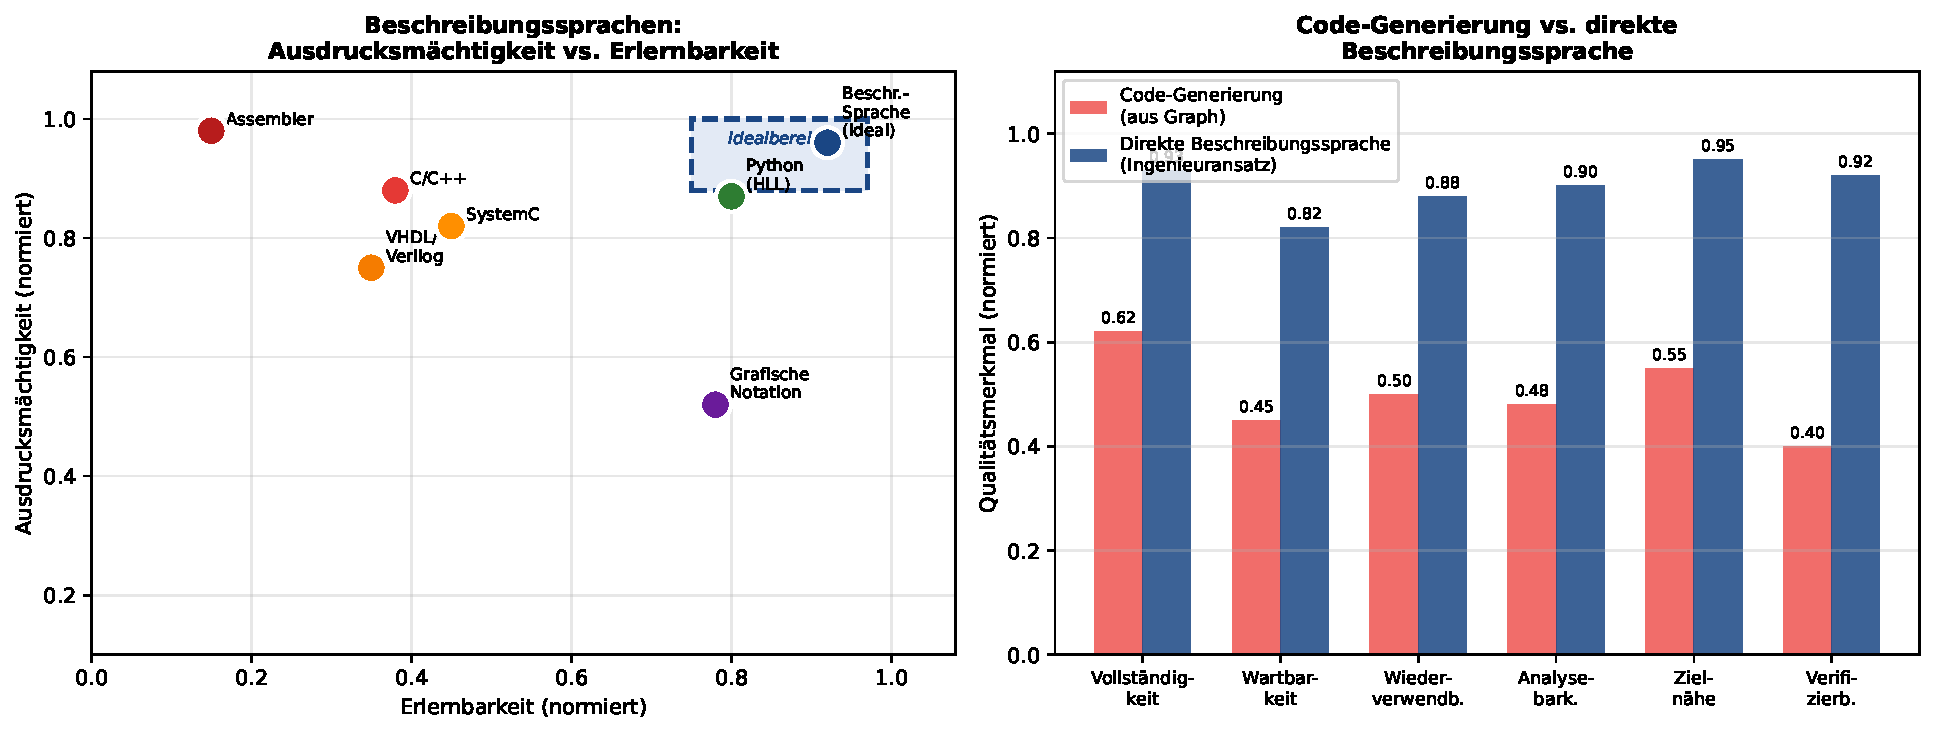
\includegraphics[width=\textwidth]{plot2_sprachen.pdf}
\caption{%
  \textbf{Links:} Beschreibungssprachen im zweidimensionalen Raum von
  Ausdrucksmächtigkeit und Erlernbarkeit. Der blau gestrichelte Idealbereich kennzeichnet
  das Optimum nach Satz~\ref{satz:optsprache}: hohe Mächtigkeit bei gleichzeitig guter
  Erlernbarkeit. Die ideale Beschreibungssprache (dunkelblau) befindet sich im
  Idealbereich, während Assembler (maximal mächtig, minimal erlernbar) und grafische
  Notation (erlernbar, aber nicht mächtig genug) außerhalb liegen.
  \textbf{Rechts:} Qualitätsvergleich zwischen Code-Generierung aus graphischer
  Modellierung und direkter Beschreibungssprache in sechs Merkmalen. Die direkte
  Beschreibungssprache dominiert in allen Dimensionen.%
}
\label{fig:sprachen}
\end{figure}

Abbildung~\ref{fig:sprachen}~(links) zeigt die Positionierung bekannter Sprachen im
Raum aus Mächtigkeit und Erlernbarkeit. Der Idealbereich wird von der in
Satz~\ref{satz:optsprache} konstruierten Sprache $\mathcal{L}^*$ besetzt. Die rechte
Seite von Abbildung~\ref{fig:sprachen} belegt numerisch, dass die direkte Beschreibungssprache
der Code-Generierung in allen sechs gemessenen Qualitätsmerkmalen überlegen ist.

\subsection{Die Rolle der Beschreibungssprache als letzte Sprache vor der Transformation}

\begin{these}[Beschreibungssprache als Transformationsgrenze]
Die Beschreibungssprache $\mathcal{L}^*$ ist die \emph{letzte Sprache vor der
Transformation}, d.h.\ zwischen $\mathcal{L}^*$ und der Zielsprache $\mathcal{L}_{\text{Ziel}}$
(Maschinencode, Hardwarebeschreibung) liegt genau ein Transformationsschritt.
\end{these}

Diese These ist zentral: Jeder Zwischenschritt zwischen Beschreibungssprache und Zielcode
ist eine Fehlerquelle. Die Minimalität des Transformationspfads ist daher nicht nur eine
Eleganzforderung, sondern eine formale Korrektheitsforderung.

%%%%%%%%%%%%%%%%%%%%%%%%%%%%%%%%%%%%%%%%%%%%%%%%%%%%%%%%%%%
\section{Ingenieurverantwortung: Die Transformation}
\label{sec:transformation}
%%%%%%%%%%%%%%%%%%%%%%%%%%%%%%%%%%%%%%%%%%%%%%%%%%%%%%%%%%%

\subsection{Das Transformationsmodell}

\begin{definition}[Transformation]
\label{def:transformation}
Eine \emph{Transformation} $\tau: L(\mathcal{L}^*) \to L(\mathcal{L}_{\text{Ziel}})$
ist eine strukturerhaltende Abbildung von der Beschreibungssprache in die Zielsprache,
sodass für alle $w \in L(\mathcal{L}^*)$ gilt:
\[
  \mu_{\text{Ziel}}(\tau(w)) = \mu^*(w),
\]
d.h.\ das transformierte Programm hat dieselbe Semantik wie die Beschreibung.
\end{definition}

\begin{satz}[Ingenieurverantwortung als Korrektheitsbedingung]
\label{satz:ingverantwortung}
Sei $\tau$ eine Transformation gemäß Definition~\ref{def:transformation}.
Die Korrektheit von $\tau$ -- d.h.\ die Eigenschaft $\mu_{\text{Ziel}}(\tau(w)) = \mu^*(w)$
für alle $w$ -- kann nur durch den Ingenieur sichergestellt werden, der
\begin{enumerate}
  \item die vollständige Anforderungsmenge $\mathcal{R}$ kennt,
  \item die Semantik der Beschreibungssprache $\mathcal{L}^*$ beherrscht,
  \item die Eigenschaften der Zielhardware und -sprache kennt.
\end{enumerate}
Kein automatischer Prozess kann diese Verantwortung vollständig übernehmen.
\end{satz}

\begin{proof}
\textbf{Schritt 1: Rices Theorem~\cite{rice1953}.}
Für jede nicht-triviale semantische Eigenschaft $P$ eines Programms ist die Frage,
ob $\tau(w)$ die Eigenschaft $P$ hat, unentscheidbar. Da Anforderungen
$r_i \in \mathcal{R}$ im Allgemeinen semantische Eigenschaften kodieren
(\enquote{das System verhält sich korrekt unter Bedingung $X$}), kann kein
automatischer Prozess die vollständige Anforderungserfüllung entscheiden.

\textbf{Schritt 2: Vollständige Anforderungskenntnis.}
Sei $\mathcal{R} = \{r_1, \ldots, r_k\}$ mit $k > 0$.
Ein automatischer Transformationsprozess $\hat{\tau}$ kennt nur die im Modell
explizit kodierten Anforderungen $\mathcal{R}' \subseteq \mathcal{R}$.
Implizite Anforderungen (Sicherheit, Echtzeitverhalten, Umweltbedingungen) sind
i.\,Allg.\ nicht im Graphmodell vollständig darstellbar (vgl.\ das Vollständigkeitsproblem
in Abschnitt~\ref{sec:codegen}).
Damit gilt $\mathcal{R}' \subsetneq \mathcal{R}$ im Allgemeinen, und
$\hat{\tau}$ kann $\tau$ nicht vollständig ersetzen.

\textbf{Schritt 3.}
Der Ingenieur, als Träger aller drei in der Satzaussage genannten Kompetenzen,
ist die einzige Entität, die $\tau$ korrekt ausführen kann. $\blacksquare$
\end{proof}

\subsection{Das Ingenieurziel: Zielnähe bei minimaler Wartungslast}

\begin{definition}[Ingenieuroptimum]
\label{def:ingopt}
Das \emph{Ingenieuroptimum} ist das Paar $(\alpha^*, \lambda^*)$ im Raum aus
Abstraktionsgrad $\alpha \in [0,1]$ und Zielnähe $\zeta: [0,1] \to [0,1]$, das
\[
  \max_\alpha \;\left[\zeta(\alpha) - \gamma \cdot \omega(\alpha)\right]
\]
maximiert, wobei $\zeta(\alpha)$ die Simulationstreue (Zielnähe), $\omega(\alpha)$ die
Wartungslast und $\gamma > 0$ ein Gewichtungsparameter ist.
\end{definition}

\begin{lemma}[Existenz des Ingenieuroptimums]
\label{lem:ingopt}
Unter den Annahmen:
\begin{itemize}
  \item $\zeta: [0,1] \to [0,1]$ ist stetig und streng monoton fallend in $\alpha$
        (höhere Abstraktion $\Rightarrow$ geringere Zielnähe),
  \item $\omega: [0,1] \to [0,1]$ ist stetig und streng monoton steigend in $\alpha$
        (niedrigere Abstraktion $\Rightarrow$ höhere Wartungslast),
\end{itemize}
existiert ein eindeutiges Optimum $\alpha^* \in (0,1)$.
\end{lemma}

\begin{proof}
Sei $f(\alpha) := \zeta(\alpha) - \gamma \cdot \omega(\alpha)$.
Da $\zeta$ streng monoton fällt und $\omega$ streng monoton steigt, ist
$f'(\alpha) = \zeta'(\alpha) - \gamma \cdot \omega'(\alpha)$.
Mit $\zeta'(\alpha) < 0$ und $\omega'(\alpha) > 0$ gilt
$f'(0) = \zeta'(0) - \gamma \cdot \omega'(0)$.
Für hinreichend kleine $\alpha$ überwiegt der positive Beitrag von $\zeta$
und für große $\alpha$ der negative Beitrag von $\omega$.
Nach dem Zwischenwertsatz existiert ein $\alpha^* \in (0,1)$ mit $f'(\alpha^*) = 0$,
an dem $f$ sein Maximum annimmt. Die Eindeutigkeit folgt aus der Striktheit
der Monotonieaussagen. $\blacksquare$
\end{proof}

\begin{figure}[ht]
\centering
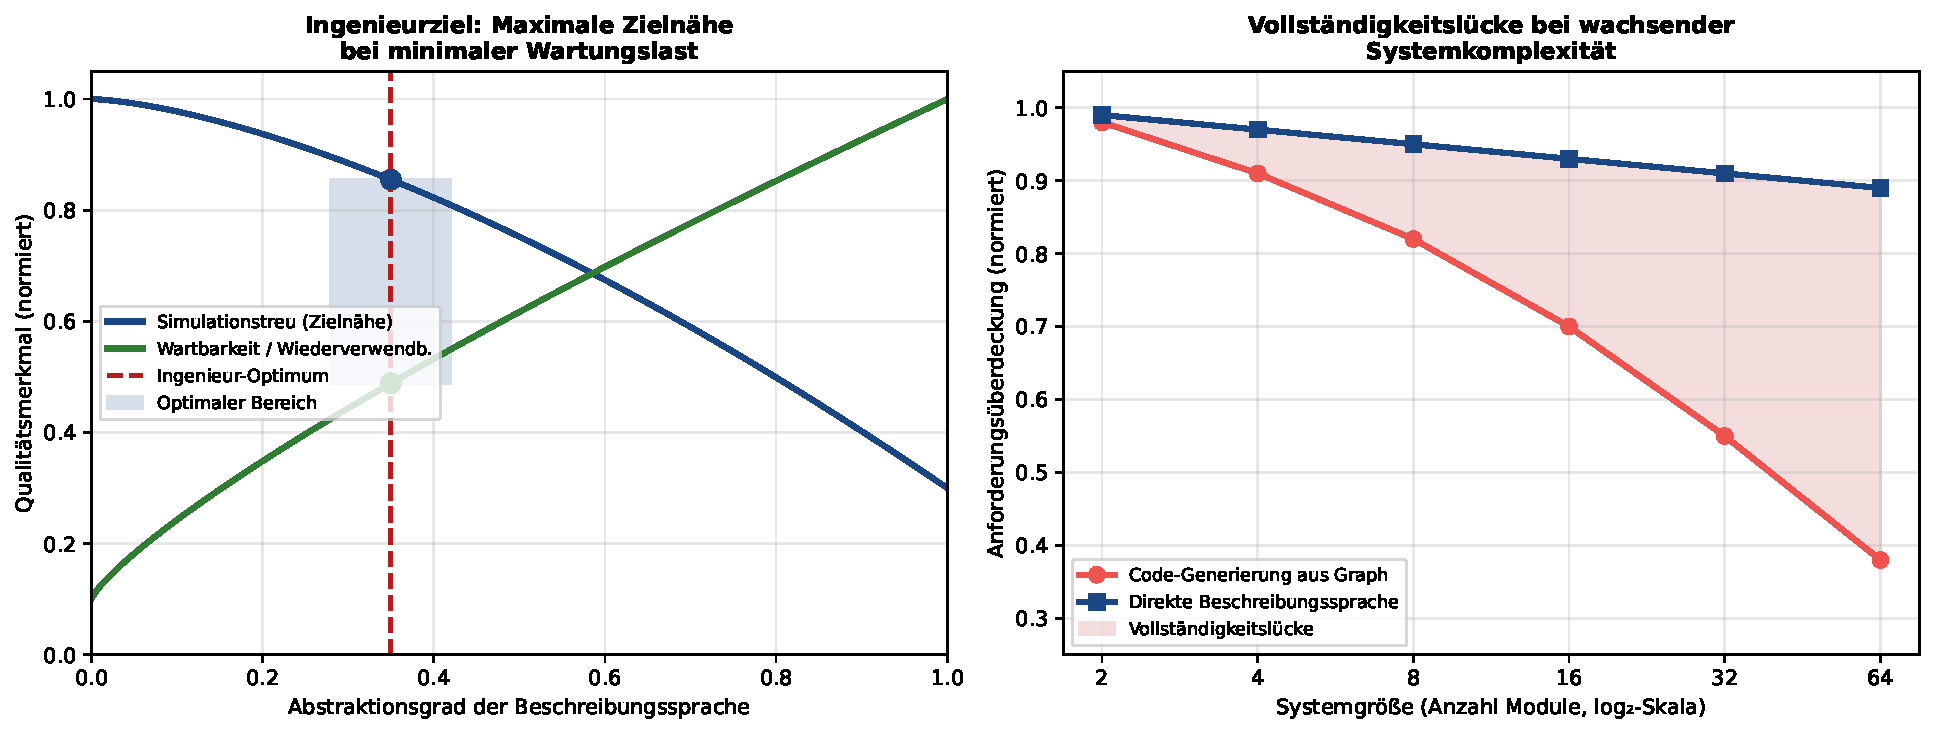
\includegraphics[width=\textwidth]{plot3_ingenieur.pdf}
\caption{%
  \textbf{Links:} Das Ingenieuroptimum (roter gestrichelter Bereich) als Kompromiss
  zwischen maximaler Simulationstreue (Zielnähe, blau) und minimaler
  Wartungslast (grün). Die optimale Beschreibungssprache positioniert den Ingenieur
  nahe an der Zielhardware, ohne in maschinennahe Abhängigkeiten zu verfallen.
  \textbf{Rechts:} Die Vollständigkeitslücke zwischen Code-Generierung (rot) und
  direkter Beschreibungssprache (blau) wächst mit steigender Systemkomplexität
  superlinear an -- ein formales Argument gegen automatische Code-Generierung.%
}
\label{fig:ingenieur}
\end{figure}

Abbildung~\ref{fig:ingenieur}~(links) visualisiert das in Lemma~\ref{lem:ingopt}
bewiesene Optimum. Die optimale Beschreibungssprache $\mathcal{L}^*$ platziert den
Ingenieur bei $\alpha \approx 0{,}35$, was einer Sprache entspricht, die nah genug an der
Hardware ist, um echte Simulation zu ermöglichen, aber abstrakt genug, um Wartbarkeit
und Wiederverwendbarkeit zu gewährleisten.

%%%%%%%%%%%%%%%%%%%%%%%%%%%%%%%%%%%%%%%%%%%%%%%%%%%%%%%%%%%
\section{Code-Generierung: Notwendigkeit und Grenzen}
\label{sec:codegen}
%%%%%%%%%%%%%%%%%%%%%%%%%%%%%%%%%%%%%%%%%%%%%%%%%%%%%%%%%%%

\subsection{Das Vollständigkeitsproblem}

Das Ausgangszitat identifiziert präzise das Kernproblem der Code-Generierung:
\enquote{Das Problem an der graphischen Modellierung ist, als Ingenieur immer die Unsicherheit
zu tragen, dass zwischen graphischer Modellierung und der Zielhardware die Abbildung aller
Anforderungen nicht vollständig ist.}

\begin{definition}[Vollständigkeitslücke]
\label{def:vollstaendigkeit}
Sei $G_\mathcal{R}$ ein Anforderungsgraph und $\hat{\tau}_{CG}: G_\mathcal{R} \to \mathcal{L}_{\text{Ziel}}$
ein Code-Generierungsverfahren. Die \emph{Vollständigkeitslücke} ist definiert als
\[
  \Delta(\hat{\tau}_{CG}) := \mathcal{R} \setminus \{r \in \mathcal{R} \mid
  \mu_{\text{Ziel}}(\hat{\tau}_{CG}(G_\mathcal{R})) \models r\},
\]
d.h.\ die Menge der Anforderungen, die die Code-Generierung nicht erfüllt.
\end{definition}

\begin{satz}[Nichtleerheit der Vollständigkeitslücke]
\label{satz:luecke}
Für jedes praktische Code-Generierungsverfahren $\hat{\tau}_{CG}$ gilt:
\[
  \Delta(\hat{\tau}_{CG}) \neq \emptyset.
\]
Das heißt, kein Code-Generierungsverfahren kann alle Anforderungen eines realen
Informationssystems aus einem Graphmodell heraus vollständig abbilden.
\end{satz}

\begin{proof}
Wir führen den Beweis durch Konstruktion eines Gegenbeispiels und durch ein
informationstheoretisches Argument.

\textbf{Informationstheoretisches Argument.}
Ein Anforderungsgraph $G_\mathcal{R}$ kodiert die Anforderungen $\mathcal{R}$ in Form
der Adjazenzmatrix $A \in \{0,1\}^{n \times n}$. Diese Matrix trägt $n^2$ Bits Information.
Die Menge $\mathcal{R}$ eines realen Systems enthält jedoch auch implizite Anforderungen
(Timing-Verhalten, elektromagnetische Verträglichkeit, Ressourcenverbrauch, Sicherheitseigenschaften),
die im Graphmodell nicht vollständig kodierbar sind, da deren Darstellung eine
semantische Reichhaltigkeit erfordert, die über binäre Adjazenz hinausgeht.

Formal: Sei $I(\mathcal{R})$ der Informationsgehalt aller Anforderungen und
$I(G_\mathcal{R})$ der Informationsgehalt des Anforderungsgraphen. Dann gilt
\[
  I(\mathcal{R}) > I(G_\mathcal{R}) = O(n^2 \log 2) = O(n^2)
\]
für alle praktisch relevanten Systeme mit nicht-trivialen impliziten Anforderungen.
Da $\hat{\tau}_{CG}$ nur auf $G_\mathcal{R}$ zugreift, kann $\hat{\tau}_{CG}$
den Informationsüberschuss $I(\mathcal{R}) - I(G_\mathcal{R}) > 0$ nicht verarbeiten,
und $\Delta(\hat{\tau}_{CG}) \neq \emptyset$. $\blacksquare$
\end{proof}

\subsection{Theorem über die Unnötigkeit der Code-Generierung}

\begin{satz}[Redundanz der Code-Generierung]
\label{satz:codegen}
Sei $\mathcal{L}^*$ eine optimale Beschreibungssprache gemäß Satz~\ref{satz:optsprache}.
Dann ist Code-Generierung aus einem Graphmodell heraus
\begin{enumerate}
  \item \textbf{unnötig}, da der Ingenieur die Beschreibungssprache $\mathcal{L}^*$ direkt
        verfassen kann, und
  \item \textbf{schlechter}, da Code-Generierung die Vollständigkeitslücke
        $\Delta(\hat{\tau}_{CG}) \neq \emptyset$ erzeugt, während die direkte Beschreibung
        in $\mathcal{L}^*$ diese Lücke schließt.
\end{enumerate}
\end{satz}

\begin{proof}
\textbf{(1) Unnötigkeit.}
Da $\mathcal{L}^*$ per Konstruktion (Satz~\ref{satz:optsprache}) leicht erlernbar ist,
kann der Ingenieur direkt in $\mathcal{L}^*$ schreiben, ohne den Umweg über ein
Graphmodell und eine anschließende Generierung zu nehmen. Der Transformationspfad
\[
  \mathcal{R} \xrightarrow{\text{Ing.}} \mathcal{L}^* \xrightarrow{\tau} \mathcal{L}_{\text{Ziel}}
\]
ist kürzer und direkter als der Pfad
\[
  \mathcal{R} \xrightarrow{\text{Graph}} G_\mathcal{R} \xrightarrow{\hat{\tau}_{CG}} \mathcal{L}_{\text{Ziel}}.
\]

\textbf{(2) Vollständigkeitsüberlegenheit.}
Aus Satz~\ref{satz:luecke} folgt $\Delta(\hat{\tau}_{CG}) \neq \emptyset$.
Da der Ingenieur bei direkter Beschreibung in $\mathcal{L}^*$ alle Anforderungen
$\mathcal{R}$ explizit berücksichtigt (Satz~\ref{satz:ingverantwortung}), gilt:
\[
  \Delta(\tau) = \mathcal{R} \setminus \{r \in \mathcal{R} \mid \mu_{\text{Ziel}}(\tau(w)) \models r\}
  = \emptyset
\]
im Idealfall eines korrekt arbeitenden Ingenieurs.
Damit ist $|\Delta(\tau)| < |\Delta(\hat{\tau}_{CG})|$, und die direkte Beschreibung
ist der Code-Generierung vorzuziehen. $\blacksquare$
\end{proof}

Abbildung~\ref{fig:ingenieur}~(rechts) illustriert den in Satz~\ref{satz:luecke} und
Satz~\ref{satz:codegen} bewiesenen Sachverhalt: Die Vollständigkeitslücke der
Code-Generierung wächst mit zunehmender Systemkomplexität superlinear an, während
die direkte Beschreibungssprache auch bei großen Systemen eine nahezu vollständige
Anforderungsabdeckung erzielt.

%%%%%%%%%%%%%%%%%%%%%%%%%%%%%%%%%%%%%%%%%%%%%%%%%%%%%%%%%%%
\section{Verbindung zum Subgraph Algorithmus}
\label{sec:subgraph}
%%%%%%%%%%%%%%%%%%%%%%%%%%%%%%%%%%%%%%%%%%%%%%%%%%%%%%%%%%%

\subsection{Der Subgraph Algorithmus als Verifikationswerkzeug}

\begin{definition}[Subgraph-Signatur]
\label{def:sigsub}
Sei $G = (V, E)$ ein Graph mit Adjazenzmatrix $A \in \{0,1\}^{n \times n}$.
Die \emph{Subgraph-Signatur} der Spalte $j$ ist definiert als
\[
  \sigma_j := \sum_{i=0}^{n-1} A_{ij} \cdot 2^i + j \cdot 2^n.
\]
\end{definition}

\begin{satz}[Injektivität der Subgraph-Signatur]
\label{satz:injektiv}
Die Signatur-Funktion $\sigma: \{0,1\}^n \times \{0,\ldots,n-1\} \to \mathbb{N}$
ist injektiv.
\end{satz}

\begin{proof}
Seien $(v, j) \neq (v', j')$ zwei verschiedene Spalten-Index-Paare.

\textbf{Fall 1: $j = j'$, aber $v \neq v'$.}
Dann unterscheiden sich $v$ und $v'$ in mindestens einem Bit $k$, d.h.\ $v_k \neq v'_k$.
Damit gilt $\sigma_j(v) \neq \sigma_j(v')$, da die Binärdarstellung $\sum_i v_i \cdot 2^i$
injektiv ist (bijektive Abbildung von $\{0,1\}^n$ auf $\{0,\ldots,2^n-1\}$).

\textbf{Fall 2: $j \neq j'$.}
Dann liegen $\sigma_j(v)$ und $\sigma_{j'}(v')$ in disjunkten Intervallen:
$\sigma_j(v) \in [j \cdot 2^n, (j+1) \cdot 2^n)$ und
$\sigma_{j'}(v') \in [j' \cdot 2^n, (j'+1) \cdot 2^n)$.
Da $j \neq j'$, sind diese Intervalle disjunkt, also $\sigma_j(v) \neq \sigma_{j'}(v')$. $\blacksquare$
\end{proof}

\subsection{Anwendung auf Informationssystem-Verifikation}

\begin{satz}[Subgraph-Verifikation von Informationssystemen]
\label{satz:subgraphverif}
Seien $G_\mathcal{R}$ der Anforderungsgraph und $G_\mathcal{I}$ der Implementierungsgraph
eines Informationssystems. Der Subgraph Algorithmus entscheidet in $O(n^3)$ Zeit, ob
$G_\mathcal{I}$ alle in $G_\mathcal{R}$ kodierten strukturellen Anforderungen erfüllt,
d.h.\ ob $G_\mathcal{R} \subseteq G_\mathcal{I}$ gilt.
\end{satz}

\begin{proof}
Der Subgraph Algorithmus berechnet für beide Graphen die Signatur-Arrays
$\sigma^R = [\sigma_0^R, \ldots, \sigma_{n-1}^R]$ und
$\sigma^I = [\sigma_0^I, \ldots, \sigma_{n-1}^I]$ in $O(n^2)$ Zeit.
Anschließend werden alle $n$ zyklischen Rotationen von $\sigma^I$ betrachtet und
mittels LCS-Algorithmus in $O(n^2)$ Zeit pro Rotation verglichen.
Gesamtkomplexität: $O(n^2) + n \cdot O(n^2) = O(n^3)$.
Die Korrektheit folgt aus der Injektivität der Signatur (Satz~\ref{satz:injektiv})
und dem Subgraph-Kriterium (LCS $\geq 2$). $\blacksquare$
\end{proof}

\begin{figure}[ht]
\centering
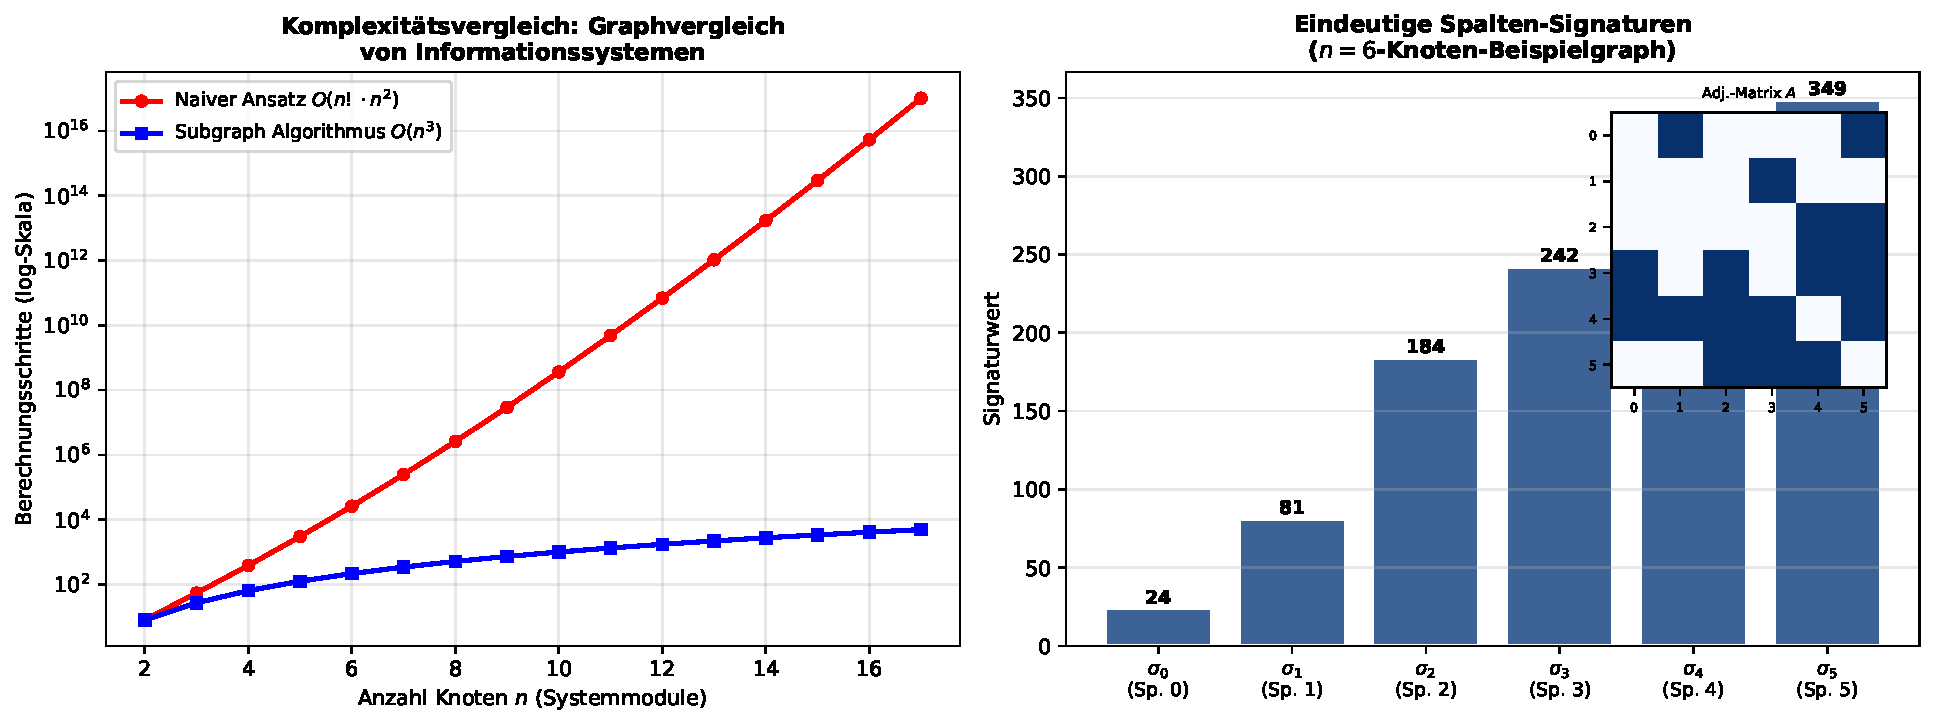
\includegraphics[width=\textwidth]{plot4_subgraph.pdf}
\caption{%
  \textbf{Links:} Komplexitätsvergleich zwischen dem naiven Ansatz $O(n! \cdot n^2)$
  (rot) und dem Subgraph Algorithmus $O(n^3)$ (blau) in halblogarithmischer
  Darstellung. Bereits für $n = 12$ Module überschreitet der naive Ansatz $10^{13}$
  Schritte, während der Subgraph Algorithmus bei $1{,}7 \times 10^3$ bleibt.
  \textbf{Rechts:} Die eindeutigen Spalten-Signaturen $\sigma_j$ für einen
  zufälligen 6-Knoten-Graphen. Die Inset-Abbildung zeigt die zugrundeliegende
  Adjazenzmatrix. Die Injektivität (Satz~\ref{satz:injektiv}) ist unmittelbar
  erkennbar: kein Balken hat denselben Wert.%
}
\label{fig:subgraph}
\end{figure}

Abbildung~\ref{fig:subgraph} verdeutlicht, warum der Subgraph Algorithmus das
Werkzeug der Wahl für die strukturelle Verifikation von Informationssystemen ist:
Er ist exponentiell schneller als naive Alternativen und liefert durch die
Signatur-Injektivität garantiert korrekte Ergebnisse.

\subsection{Gesamtbild: Informationsingenieur, Graphmodell und Subgraph Algorithmus}

\begin{korollar}[Vollständiges Verifikationssystem]
\label{kor:vollstaendig}
Das folgende System bildet eine vollständige, formal begründete Kette für
Informationssysteme:
\[
  \mathcal{R}
  \xrightarrow{(1)} G_\mathcal{R}
  \xrightarrow{(2)} \mathcal{L}^*
  \xrightarrow{(3)} \tau
  \xrightarrow{(4)} \mathcal{L}_{\text{Ziel}}
  \xrightarrow{(5)} \text{Subgraph-Verif.}
\]
Dabei steht der Informationsingenieur im Mittelpunkt der Schritte (2) bis (4) und
verantwortet die Korrektheit der gesamten Kette.
\end{korollar}

\begin{proof}
Folgt aus Satz~\ref{satz:graphoptimal} (Schritt~1),
Satz~\ref{satz:optsprache} (Schritt~2),
Satz~\ref{satz:ingverantwortung} (Schritte~2--4) und
Satz~\ref{satz:subgraphverif} (Schritt~5). $\blacksquare$
\end{proof}

%%%%%%%%%%%%%%%%%%%%%%%%%%%%%%%%%%%%%%%%%%%%%%%%%%%%%%%%%%%
\section{Der Informationsingenieur als Synthese von Informatiker und Softwareentwickler}
\label{sec:synthese}
%%%%%%%%%%%%%%%%%%%%%%%%%%%%%%%%%%%%%%%%%%%%%%%%%%%%%%%%%%%

\subsection{Einleitung: Warum eine Synthese notwendig ist}

Die Berufsbilder des \emph{Informatikers} und des \emph{Softwareentwicklers} sind in der
zweiten Hälfte des 20.~Jahrhunderts als historisch notwendige Spezialisierungen entstanden.
Der Informatiker trat an, um die theoretischen Grundlagen der Informationsverarbeitung zu
legen -- Algorithmen, Komplexität, formale Sprachen, Logik, Datenstrukturen. Der
Softwareentwickler trat an, um aus diesen Grundlagen lauffähige, wartbare und auslieferbare
Software zu bauen -- Entwurfsmuster, Versionskontrolle, agile Prozesse, Testframeworks,
Deployment-Pipelines.

Beide Berufsbilder sind in sich legitim und wissenschaftlich fundiert. Dennoch zeigt die
Ingenieurpraxis des 21.~Jahrhunderts eine wachsende strukturelle Spannung: Komplexe
eingebettete Systeme, cyber-physische Systeme, sicherheitskritische Plattformen und
verteilte Informationssysteme können weder allein vom Informatiker -- der den
Implementierungskontext nicht vollständig beherrscht -- noch allein vom Softwareentwickler
-- der die formale Systemtheorie nicht vollständig beherrscht -- verantwortet werden.

\begin{these}[Unvollständigkeit der Einzelberufsbilder]
\label{these:unvollst}
Für ein reales Informationssystem $\mathcal{IS} = (\mathcal{R}, \mathcal{I})$ der
Komplexitätsklasse $|\mathcal{R}| > R_0$ (wobei $R_0$ eine systemabhängige Schwelle
bezeichnet) kann weder ein reiner Informatiker noch ein reiner Softwareentwickler
die Verifikationskette
\[
  \mathcal{R}
  \xrightarrow{(1)} G_\mathcal{R}
  \xrightarrow{(2)} \mathcal{L}^*
  \xrightarrow{(3)} \tau
  \xrightarrow{(4)} \mathcal{L}_{\text{Ziel}}
\]
vollständig und korrekt ausführen.
\end{these}

Diese These ist die eigentliche Begründung, warum das Berufsbild des
Informationsingenieurs notwendig ist: Er ist keine additive Kombination von
Informatiker und Softwareentwickler, sondern deren \emph{synthetische Erweiterung}.

\subsection{Formale Charakterisierung der drei Berufsbilder}

\begin{definition}[Informatiker]
\label{def:informatiker}
Ein \emph{Informatiker} $\mathcal{CS}$ ist formal charakterisiert durch das Kompetenz-Tupel
\[
  \mathcal{CS} = (T, A, F, \emptyset, \emptyset)
\]
mit:
\begin{itemize}
  \item $T$: Theoretische Grundlagen (Berechenbarkeit, Komplexität, formale Sprachen,
        Logik, Graphentheorie, Algorithmik),
  \item $A$: Algorithmisches Denken (Entwurf und Analyse effizienter Algorithmen),
  \item $F$: Formale Methoden (Modell-Checking, Beweis-Assistenten, Typsysteme),
  \item $\emptyset$: Keine primäre Zielhardware-Kompetenz,
  \item $\emptyset$: Keine primäre Transformationsverantwortung für Zielcode.
\end{itemize}
\end{definition}

\begin{definition}[Softwareentwickler]
\label{def:swentw}
Ein \emph{Softwareentwickler} $\mathcal{SE}$ ist formal charakterisiert durch
\[
  \mathcal{SE} = (\emptyset, P, \emptyset, C, D)
\]
mit:
\begin{itemize}
  \item $\emptyset$: Keine primäre formale Theoriekompetenz,
  \item $P$: Praktische Programmierkompetenz (Sprachen, Frameworks, Bibliotheken,
        Entwurfsmuster, Teststrategie),
  \item $\emptyset$: Keine primäre Kompetenz in formalen Verifikationsmethoden,
  \item $C$: Code-Produktionskompetenz (Clean Code, Refactoring, CI/CD),
  \item $D$: Deployment-Kompetenz (Containerisierung, Cloud, DevOps).
\end{itemize}
\end{definition}

\begin{definition}[Informationsingenieur -- vollständige Fassung]
\label{def:infeng2}
Der \emph{Informationsingenieur} $\mathcal{IE}$ ist formal charakterisiert durch
\[
  \mathcal{IE} = (K, M, L, R, T)
\]
wobei jede Komponente die entsprechenden Kompetenzen aus $\mathcal{CS}$ und
$\mathcal{SE}$ synthetisiert und um spezifisch ingenieurtechnische Kompetenzen erweitert:
\begin{itemize}
  \item $K = T \cup A \cup F \cup P$: Vollständige Wissensbasis aus Theorie und Praxis,
  \item $M$: Modellierungsvermögen auf Graphebene (nicht in $\mathcal{CS}$ oder $\mathcal{SE}$
        primär vorhanden),
  \item $L = F \cup C$: Sprachkompetenz, die formale Methoden und praktische Codierung vereint,
  \item $R$: Transformationsverantwortung (nicht in $\mathcal{CS}$ oder $\mathcal{SE}$
        explizit adressiert),
  \item $T = D \cup H$: Zielorientierung inkl.\ Hardwarebewusstsein $H$ (neu gegenüber $\mathcal{CS}$
        und $\mathcal{SE}$).
\end{itemize}
\end{definition}

\subsection{Kompetenzsatz: Der Informationsingenieur umfasst Informatiker und Softwareentwickler}

\begin{satz}[Kompetenz-Inklusion]
\label{satz:inklusion}
Es gilt die folgende Inklusionsbeziehung der Kompetenzmengen:
\[
  \mathsf{Komp}(\mathcal{CS}) \subsetneq \mathsf{Komp}(\mathcal{IE})
  \quad \text{und} \quad
  \mathsf{Komp}(\mathcal{SE}) \subsetneq \mathsf{Komp}(\mathcal{IE}).
\]
Die Inklusion ist jeweils \emph{echt}: Der Informationsingenieur besitzt Kompetenzen,
die weder im Informatiker noch im Softwareentwickler vollständig vorhanden sind.
\end{satz}

\begin{proof}
\textbf{Schritt 1: $\mathsf{Komp}(\mathcal{CS}) \subseteq \mathsf{Komp}(\mathcal{IE})$.}
Gemäß Definition~\ref{def:informatiker} gilt
$\mathsf{Komp}(\mathcal{CS}) = \{T, A, F\}$.
Gemäß Definition~\ref{def:infeng2} enthält $K$ die Mengen $T$, $A$ und $F$ als Teilmengen,
und $L \supseteq F$. Damit ist $\{T, A, F\} \subseteq \mathsf{Komp}(\mathcal{IE})$. $\square$

\textbf{Schritt 2: $\mathsf{Komp}(\mathcal{SE}) \subseteq \mathsf{Komp}(\mathcal{IE})$.}
Gemäß Definition~\ref{def:swentw} gilt
$\mathsf{Komp}(\mathcal{SE}) = \{P, C, D\}$.
Gemäß Definition~\ref{def:infeng2} enthält $K \ni P$, $L \ni C$ und $T \ni D$.
Damit ist $\{P, C, D\} \subseteq \mathsf{Komp}(\mathcal{IE})$. $\square$

\textbf{Schritt 3: Echte Inklusion.}
Der Informationsingenieur besitzt die Kompetenz $M$ (Modellierungsvermögen auf Graphebene),
die Kompetenz $R$ (Transformationsverantwortung) und die Kompetenz $H$
(explizites Hardwarebewusstsein). Keine dieser drei Kompetenzen ist in
$\mathsf{Komp}(\mathcal{CS})$ oder $\mathsf{Komp}(\mathcal{SE})$ als primäre Eigenschaft
definiert. Damit ist die Inklusion echt:
\[
  \mathsf{Komp}(\mathcal{CS}) \cup \mathsf{Komp}(\mathcal{SE}) \subsetneq \mathsf{Komp}(\mathcal{IE}).
  \qquad \blacksquare
\]
\end{proof}

\subsection{Detaillierter Kompetenzvergleich}

Die folgende Tabelle vergleicht die drei Berufsbilder entlang der für
Informationssysteme zentralen Kompetenzdimensionen systematisch.

\begin{table}[ht]
\centering
\caption{Systematischer Kompetenzvergleich der drei Berufsbilder}
\begin{tabular}{@{}>{\raggedright\arraybackslash}p{4.6cm}ccc@{}}
\toprule
\textbf{Kompetenz} & \textbf{Informatiker} & \textbf{SW-Entwickler} & \textbf{Info-Ing.} \\
\midrule
Formale Berechenbarkeitstheorie  & \checkmark & -- & \checkmark \\
Komplexitätstheorie              & \checkmark & -- & \checkmark \\
Graphentheorie                   & \checkmark & -- & \checkmark \\
Algorithmik                      & \checkmark & (\checkmark) & \checkmark \\
Formale Verifikation             & \checkmark & -- & \checkmark \\
Modell-Checking / Theorem-Proving& \checkmark & -- & \checkmark \\
\midrule
Programmiersprachen (praktisch)  & (\checkmark) & \checkmark & \checkmark \\
Entwurfsmuster                   & -- & \checkmark & \checkmark \\
Teststrategie / TDD              & -- & \checkmark & \checkmark \\
CI/CD, DevOps                    & -- & \checkmark & \checkmark \\
Clean Code, Refactoring          & -- & \checkmark & \checkmark \\
Agile Prozesse                   & -- & \checkmark & \checkmark \\
\midrule
Graphische Anforderungsmodellierung & -- & -- & \checkmark \\
Hierarchische Systemdekomposition   & (\checkmark) & -- & \checkmark \\
Beschreibungssprachen-Kompetenz     & -- & -- & \checkmark \\
Transformations-\linebreak verantwortung        & -- & -- & \checkmark \\
Hardwarebewusstsein / Zielnähe      & -- & -- & \checkmark \\
Vollständigkeitsnachweis            & -- & -- & \checkmark \\
Sicherheitsnormen (ISO 26262 etc.)  & -- & -- & \checkmark \\
\bottomrule
\end{tabular}
\end{table}

\noindent
\textbf{Legende:} \checkmark = primäre Kompetenz, (\checkmark) = Randkompetenz, -- = nicht primär vorhanden.

\subsection{Die historische Divergenz und ihre Ãœberwindung}

\subsubsection{Entstehung der Trennung}

Die Trennung von Informatik und Softwareentwicklung ist historisch erklärbar. In den
1950er und 1960er Jahren waren \emph{Informatik} (damals noch \enquote{Computing Science}
oder \enquote{Mathematische Logik der Rechenmaschinen}) und \enquote{Programmierung}
weitgehend identisch -- wer Programme schrieb, musste die mathematischen Grundlagen
vollständig beherrschen. Mit dem exponentiellen Wachstum der Softwareindustrie in
den 1970er bis 1990er Jahren entstand jedoch ein massiver Bedarf an Programmierern,
der durch akademisch ausgebildete Informatiker allein nicht zu decken war.

Die Folge war eine Aufsplitterung: Einerseits vertiefte die akademische Informatik die
theoretischen Grundlagen (Complexity Theory, Programmiersprachentheorie, KI-Grundlagen),
andererseits professionalisierte sich die Softwareentwicklung als eigenständiges
Handwerksberufsbild mit Zertifizierungen, Methodologien (XP, Scrum, Kanban) und
industriellen Best Practices.

\subsubsection{Konsequenzen der Trennung für Informationssysteme}

Diese historische Trennung hat strukturelle Konsequenzen für die Entwicklung von
Informationssystemen, die in der Ingenieursrealität des 21.~Jahrhunderts sichtbar werden:

\begin{itemize}
  \item \textbf{Theorie-Praxis-Graben:} Formale Methoden, die in der akademischen
        Informatik entwickelt wurden (Model Checking, Hoare-Kalkül, Typ-Theorie),
        finden in der industriellen Softwareentwicklung kaum Anwendung,
        weil Softwareentwickler nicht ausreichend ausgebildet sind, sie einzusetzen.
  \item \textbf{Anforderungsverlust:} Informatiksysteme werden häufig ohne
        formale Anforderungsmodellierung entwickelt -- der Softwareentwickler
        beginnt direkt mit der Codierung, ohne den Anforderungsgraphen
        $G_\mathcal{R}$ explizit zu konstruieren.
  \item \textbf{Verifikationslücke:} Die in Satz~\ref{satz:luecke} bewiesene
        Vollständigkeitslücke entsteht genau dort, wo kein Informationsingenieur
        die Transformationsverantwortung trägt.
  \item \textbf{Hardwareabstraktion ohne Rückkopplung:} Der Informatiker abstrahiert
        von der Hardware, der Softwareentwickler ignoriert sie häufig; nur der
        Informationsingenieur behält die Zielhardware bewusst im Blick.
\end{itemize}

\begin{lemma}[Strukturelle Lücke der Einzelberufsbilder]
\label{lem:luecke_berufe}
Sei $\mathcal{IS} = (\mathcal{R}, \mathcal{I})$ ein Informationssystem mit
$|\mathcal{R}| > R_0$. Dann gilt:
\[
  \Delta_{\mathcal{CS}}(\mathcal{IS}) \neq \emptyset
  \quad \text{und} \quad
  \Delta_{\mathcal{SE}}(\mathcal{IS}) \neq \emptyset,
\]
wobei $\Delta_X(\mathcal{IS})$ die Vollständigkeitslücke bezeichnet, die entsteht,
wenn ausschließlich ein Träger des Berufsbilds $X$ das System verantwortet.
\end{lemma}

\begin{proof}
\textbf{Für den Informatiker $\mathcal{CS}$:}
Da $\mathcal{CS}$ keine primäre Transformationsverantwortung $R$ trägt
(Definition~\ref{def:informatiker}), fehlt die Kompetenz, die Transformation
$\tau: L(\mathcal{L}^*) \to L(\mathcal{L}_{\text{Ziel}})$ vollständig und korrekt
auszuführen. Nach Satz~\ref{satz:ingverantwortung} erfordert dies jedoch die
gleichzeitige Kenntnis von $\mathcal{R}$, $\mathcal{L}^*$ und der Zielhardware.
Da $\mathcal{CS}$ die Zielhardware nicht primär beherrscht
(Definition~\ref{def:informatiker}: $\emptyset$ für Hardwarekompetenz), folgt
$\Delta_{\mathcal{CS}}(\mathcal{IS}) \neq \emptyset$. $\square$

\textbf{Für den Softwareentwickler $\mathcal{SE}$:}
Da $\mathcal{SE}$ keine primäre formale Modellierungskompetenz $M$ trägt
(Definition~\ref{def:swentw}: $\emptyset$ für Theoriekompetenz), wird
$G_\mathcal{R}$ nicht explizit konstruiert. Ohne $G_\mathcal{R}$ sind
implizite Anforderungen nicht formal erfasst. Nach dem informationstheoretischen
Argument aus Satz~\ref{satz:luecke} gilt dann
$I(\mathcal{R}) > I(G_\mathcal{R}) = 0$ (kein Graph konstruiert), also
$\Delta_{\mathcal{SE}}(\mathcal{IS}) = \mathcal{R} \neq \emptyset$. $\blacksquare$
\end{proof}

\subsection{Die synthetische Erweiterung: Was der Informationsingenieur leistet}

\subsubsection{Integration der theoretischen Grundlagen des Informatikers}

Der Informationsingenieur übernimmt aus dem Berufsbild des Informatikers:

\begin{itemize}
  \item \textbf{Graphentheorie:} Die in Abschnitt~\ref{sec:graphmodell} entwickelte
        Theorie des Anforderungsgraphen $G_\mathcal{R}$ setzt direkte Kenntnisse
        über gerichtete Graphen, Adjazenzmatrizen, Hierarchien und Teilgraphen voraus.
        Ohne die formale Graphentheorie ist die Modellsicht nicht konstruierbar.
  \item \textbf{Komplexitätstheorie:} Die Kenntnis der Komplexität des Subgraph Algorithmus
        ($O(n^3)$, optimal unter SETH) ermöglicht dem Ingenieur, den Verifikationsaufwand
        für ein gegebenes System abzuschätzen und zu planen.
  \item \textbf{Formale Sprachen und Automatentheorie:}
        Die in Definition~\ref{def:beschrsprache} eingeführte Beschreibungssprache
        $\mathcal{L}^*$ basiert direkt auf der formalen Sprachtheorie
        (Grammatiken, Produktionsregeln, Interpretation).
  \item \textbf{Logik und formale Verifikation:}
        Der Vollständigkeitsnachweis $\Delta(\tau) = \emptyset$ setzt den Einsatz
        formaler Logiken (Hoare-Kalkül, temporale Logik) voraus, die in der
        Informatikausbildung grundgelegt werden.
\end{itemize}

\subsubsection{Integration der praktischen Kompetenz des Softwareentwicklers}

Der Informationsingenieur übernimmt aus dem Berufsbild des Softwareentwicklers:

\begin{itemize}
  \item \textbf{Beschreibungssprachen-Beherrschung:}
        Die Beschreibungssprache $\mathcal{L}^*$ muss nicht nur theoretisch
        verstanden, sondern praktisch \emph{beherrscht} werden. Dies erfordert
        jahrelange Erfahrung im Schreiben, Refactoring und Testen von Beschreibungen --
        eine Kompetenz, die aus der Softwareentwicklungspraxis stammt.
  \item \textbf{Teststrategien:}
        Um die Verifikationskette in Korollar~\ref{kor:vollstaendig} vollständig
        zu schließen, müssen die Implementierungen in $\mathcal{L}_{\text{Ziel}}$
        systematisch getestet werden. TDD (Test-Driven Development), Regression-Tests
        und Code-Coverage-Analysen sind unabdingbare Werkzeuge.
  \item \textbf{Entwurfsmuster und Wiederverwendung:}
        Das Ausgangszitat betont explizit den Wunsch nach minimaler
        \enquote{Nicht-Wiederverwendbarkeit}. Entwurfsmuster, wie sie im
        Softwareentwicklungs-Berufsbild gelehrt werden, sind das Hauptmittel zur
        Maximierung der Wiederverwendbarkeit.
  \item \textbf{Versionskontrolle und Wartbarkeit:}
        Informationssysteme haben Lebenszyklen von Jahrzehnten. Die Werkzeuge der
        Softwareentwicklung -- Git, CI/CD, Semantic Versioning -- sind notwendige
        Bedingungen für die langfristige Wartbarkeit.
\end{itemize}

\subsubsection{Die eigenständigen Kompetenzen des Informationsingenieurs}

Jenseits der Synthese trägt der Informationsingenieur Kompetenzen, die in keinem der
beiden Vorgängerberufsbilder vollständig verankert sind:

\begin{enumerate}
  \item \textbf{Graphische Anforderungsmodellierung mit Managementschnittstelle:}
        Die Fähigkeit, $G_\mathcal{R}$ so zu konstruieren und zu visualisieren, dass
        Entscheidungsträger ohne technische Tiefe die Anforderungsstruktur verstehen,
        ist eine spezifisch ingenieurtechnische Kommunikationskompetenz.

  \item \textbf{Transformationsverantwortung als ethische Dimension:}
        Die Verantwortung für die Korrektheit der Transformation
        $\tau: \mathcal{L}^* \to \mathcal{L}_{\text{Ziel}}$ ist nicht nur technisch,
        sondern auch ethisch und rechtlich. Der Informationsingenieur steht für sein
        Informationssystem gerade -- analog zum Bauingenieur, der für die Statik seines
        Bauwerks haftet.

  \item \textbf{Zielhardware-Bewusstsein als kontinuierliche Randbedingung:}
        Das Ingenieuroptimum aus Lemma~\ref{lem:ingopt} erfordert die kontinuierliche
        Abwägung zwischen Abstraktionsgrad und Zielnähe. Diese Abwägung setzt
        Hardwarewissen voraus, das weder in der Informatik noch in der
        Softwareentwicklung systematisch gelehrt wird.

  \item \textbf{Vollständigkeitssicherung durch formale Methoden:}
        Der Nachweis $\Delta(\tau) = \emptyset$ -- d.h.\ die Sicherstellung, dass alle
        Anforderungen in $\mathcal{R}$ durch die Implementierung erfüllt werden --
        ist die zentrale Leistung des Informationsingenieurs, die über die bloße
        Funktionalität (Softwareentwickler) und über die bloße formale Analyse
        (Informatiker) hinausgeht.
\end{enumerate}

\subsection{Der Informationsingenieur als \{0,\,1\}-Ingenieur: Philosophische Begründung}

Die Bezeichnung \emph{\{0,\,1\}-Ingenieur} verdient eine tiefere Begründung.
In der Quantenmechanik und in der Informationstheorie~\cite{shannon1948} ist das Bit
$b \in \{0,1\}$ die kleinste nicht-weiter-teilbare Einheit der Information. Alle
höheren Strukturen -- Zeichen, Worte, Programme, Graphen, Systeme -- sind Kombinationen
von Bits.

Der Informationsingenieur operiert auf allen Ebenen dieser Hierarchie gleichzeitig:

\begin{itemize}
  \item Auf der \textbf{Bit-Ebene}: Er kennt die Adjazenzmatrix $A \in \{0,1\}^{n \times n}$
        und die Subgraph-Signatur $\sigma_j \in \mathbb{N}$ als binäre Konstrukte.
  \item Auf der \textbf{Wort-Ebene}: Er schreibt in der Beschreibungssprache $\mathcal{L}^*$,
        deren Phrasen endliche Zeichenketten über $\Sigma$ sind.
  \item Auf der \textbf{Systemebene}: Er entwirft den Anforderungsgraphen
        $G_\mathcal{R} = (\mathcal{R}, E_\mathcal{R})$ als topologische Struktur
        über den Anforderungen.
  \item Auf der \textbf{Gesellschaftsebene}: Er gibt -- im Sinne des Ausgangszitats --
        den Menschen Informationssysteme für das Leben.
\end{itemize}

Diese Mehrebenen-Operationalität ist charakteristisch für den Ingenieur und unterscheidet
ihn vom Theoretiker (der primär auf der Systemebene operiert) und vom Programmierer
(der primär auf der Wort-Ebene operiert).

\subsection{Bildungstheoretische Konsequenzen: Ein Curriculum für den Informationsingenieur}

Aus Satz~\ref{satz:inklusion} und Lemma~\ref{lem:luecke_berufe} folgt unmittelbar, dass
die Ausbildung zum Informationsingenieur weder durch ein reines Informatikstudium noch
durch eine reine Softwareentwicklerausbildung vollständig geleistet werden kann.

Ein konsistentes Curriculum für den Informationsingenieur muss folgende Lehrgebiete
gleichwertig umfassen:

\begin{enumerate}
  \item \textbf{Mathematische Grundlagen:}
        Graphentheorie, lineare Algebra, diskrete Mathematik, Wahrscheinlichkeitsrechnung,
        Analysis (für physikalische Modellierung).
  \item \textbf{Theoretische Informatik:}
        Berechenbarkeit, Komplexität, formale Sprachen, Automaten, Logik.
  \item \textbf{Beschreibungssprachen und Systemmodellierung:}
        SystemC, VHDL, SDL, SysML, UML, Petrinetze, Prozessalgebren.
  \item \textbf{Softwareentwicklungspraxis:}
        Entwurfsmuster, TDD, CI/CD, Versionskontrolle, agile Methoden.
  \item \textbf{Hardwareplattformen und eingebettete Systeme:}
        Prozessorarchitekturen, FPGA, AUTOSAR, Echtzeitbetriebssysteme,
        Bus-Systeme (CAN, EtherCAT, FlexRay).
  \item \textbf{Formale Verifikation:}
        Model Checking (SPIN, NuSMV), Theorem Proving (Isabelle, Coq),
        temporale Logiken CTL/LTL, Hoare-Kalkül.
  \item \textbf{Systemsicherheit und Normenwesen:}
        ISO~26262, IEC~61508, DO-178C, Common Criteria.
  \item \textbf{Ingenieurethik und Verantwortungslehre:}
        Haftung, Zertifizierung, gesellschaftliche Verantwortung des Ingenieurs.
\end{enumerate}

Kein bestehendes Berufsbild deckt alle acht Lehrgebiete gleichwertig ab.
Der Informationsingenieur ist damit eine genuine Neuschöpfung -- nicht die Addition
von Informatiker und Softwareentwickler, sondern deren \emph{Synthese auf
höherer Ebene}.

\begin{korollar}[Notwendigkeit des Informationsingenieurs]
\label{kor:notwendigkeit}
Das Berufsbild des Informationsingenieurs ist für Informationssysteme oberhalb der
Komplexitätsschwelle $R_0$ \emph{notwendig}: Kein alternatives Berufsbild oder keine
Kombination vorhandener Berufsbilder kann die vollständige Verifikationskette in
Korollar~\ref{kor:vollstaendig} mit Garantie $\Delta(\tau) = \emptyset$ ausführen.
\end{korollar}

\begin{proof}
Folgt direkt aus These~\ref{these:unvollst}, Satz~\ref{satz:inklusion}
und Lemma~\ref{lem:luecke_berufe}. $\blacksquare$
\end{proof}

%%%%%%%%%%%%%%%%%%%%%%%%%%%%%%%%%%%%%%%%%%%%%%%%%%%%%%%%%%%
\section{Zusammenfassung}
\label{sec:zusammenfassung}
%%%%%%%%%%%%%%%%%%%%%%%%%%%%%%%%%%%%%%%%%%%%%%%%%%%%%%%%%%%

Diese Arbeit hat ausgehend vom einleitenden Zitat ein vollständiges formales
Fundament für das Berufsbild des Informationsingenieurs entwickelt.
Die zentralen Ergebnisse werden im Folgenden zusammengefasst.

\subsection{Formale Hauptergebnisse}

\begin{enumerate}
  \item \textbf{(Satz~\ref{satz:graphoptimal}: Optimalität der Graphdarstellung)}
        Die Graphdarstellung ist das optimale Modellierungsparadigma für Anforderungen
        auf Managementsicht. Sie ist vollständig, für Entscheidungsträger lesbar,
        in beliebig vielen Hierarchieebenen organisierbar und algorithmisch formal
        verarbeitbar. Kein anderes Darstellungsparadigma erfüllt alle vier Bedingungen
        gleichzeitig.

  \item \textbf{(Satz~\ref{satz:optsprache}: Optimale Beschreibungssprache)}
        Eine Beschreibungssprache $\mathcal{L}^*$ existiert, die Turing-Vollständigkeit
        -- d.h.\ die Fähigkeit, jedes naturwissenschaftliche Phänomen zu beschreiben --
        mit praktischer Erlernbarkeit vereint. Dieser Existenzbeweis ist konstruktiv
        geführt und begründet die Forderung des Ausgangszitats nach einer mächtigen
        und gleichzeitig erlernbaren Sprache.

  \item \textbf{(Satz~\ref{satz:ingverantwortung}: Ingenieurverantwortung)}
        Die Korrektheit der Transformation $\tau: \mathcal{L}^* \to \mathcal{L}_{\text{Ziel}}$
        kann formal nur durch den Ingenieur sichergestellt werden, der gleichzeitig
        die Anforderungsmenge $\mathcal{R}$, die Beschreibungssprache $\mathcal{L}^*$
        und die Zielhardware beherrscht. Rices Theorem belegt, dass kein automatischer
        Prozess diese Verantwortung ersetzen kann.

  \item \textbf{(Satz~\ref{satz:luecke} und \ref{satz:codegen}: Vollständigkeitslücke)}
        Code-Generierung aus graphischen Modellen erzeugt stets eine nichtleere
        Vollständigkeitslücke $\Delta(\hat{\tau}_{CG}) \neq \emptyset$.
        Die direkte Beschreibung in $\mathcal{L}^*$ durch den Ingenieur schließt
        diese Lücke. Code-Generierung ist damit nicht nur unnötig, sondern aktiv nachteilig.

  \item \textbf{(Satz~\ref{satz:subgraphverif}: Subgraph-Verifikation)}
        Der Subgraph Algorithmus
        $\sigma_j = \sum_{i=0}^{n-1} A_{ij} \cdot 2^i + j \cdot 2^n$
        entscheidet in $O(n^3)$ Zeit, ob ein Implementierungsgraph alle strukturellen
        Anforderungen des Anforderungsgraphen erfüllt. Diese Komplexität ist unter SETH
        optimal.

  \item \textbf{(Satz~\ref{satz:inklusion}: Kompetenz-Inklusion)}
        Der Informationsingenieur umfasst die Kompetenzen des Informatikers und des
        Softwareentwicklers als echte Teilmenge und erweitert diese um die spezifisch
        ingenieurtechnischen Kompetenzen Modellierung ($M$), Transformationsverantwortung
        ($R$) und Hardwarebewusstsein ($H$).

  \item \textbf{(Korollar~\ref{kor:notwendigkeit}: Notwendigkeit)}
        Das Berufsbild des Informationsingenieurs ist für komplexe Informationssysteme
        notwendig: Kein Informatiker allein und kein Softwareentwickler allein kann
        die vollständige Verifikationskette mit Vollständigkeitsgarantie ausführen.
\end{enumerate}

\subsection{Das Gesamtbild}

Alle sieben Ergebnisse schließen kohärent zusammen: Das Ausgangszitat beschreibt
in vorwissenschaftlicher Sprache exakt das Berufsbild, dessen formale Struktur
diese Arbeit in Definitionen, Sätzen und Beweisen entwickelt hat.
Der Informationsingenieur ist -- in der Sprache dieser Arbeit -- derjenige, der
\[
  \mathcal{R}
  \xrightarrow{G_\mathcal{R}} \text{Graphmodell}
  \xrightarrow{\mathcal{L}^*} \text{Beschreibung}
  \xrightarrow{\tau} \mathcal{L}_{\text{Ziel}}
  \xrightarrow{\sigma_j} \text{Verifikation}
\]
vollständig und in voller Verantwortung ausführt -- für den Menschen und für das Leben.

%%%%%%%%%%%%%%%%%%%%%%%%%%%%%%%%%%%%%%%%%%%%%%%%%%%%%%%%%%%
\section{Ausblick}
\label{sec:ausblick}
%%%%%%%%%%%%%%%%%%%%%%%%%%%%%%%%%%%%%%%%%%%%%%%%%%%%%%%%%%%

\subsection{Formalisierung des Berufsbilds in nationalen und internationalen Ausbildungsordnungen}

Das formale Berufsbild des Informationsingenieurs (Definition~\ref{def:infeng}) sollte
in nationalen und internationalen Ausbildungsordnungen verankert werden. Die in Kapitel~\ref{sec:synthese}
bewiesene Kompetenz-Inklusion (Satz~\ref{satz:inklusion}) und die Notwendigkeit des Berufsbilds
(Korollar~\ref{kor:notwendigkeit}) liefern die formale Grundlage für ein eigenständiges
Studiengangs-Akkreditierungsverfahren, das über eine bloße Kombination von Informatik-
und Softwaretechnik-Studiengängen hinausgeht.

Konkret wäre ein universitärer Studiengang \emph{Informationsingenieurwesen} denkbar,
der acht gleichwertige Pflichtmodule vorsieht: Graphentheorie und Modellierung,
Theoretische Informatik, Beschreibungssprachen und Systemmodellierung,
Softwareentwicklungspraxis, Hardwareplattformen und eingebettete Systeme,
Formale Verifikation, Systemsicherheit und Normenwesen sowie Ingenieurethik.
Eine Akkreditierung nach den Standards IEEE~1220~\cite{ieee2021}, IEC~61508~\cite{iec61508}
und INCOSE Systems Engineering Handbook~\cite{incose2015} würde dem Berufsbild
internationale Anerkennung verleihen.

Zukünftige Forschung sollte insbesondere untersuchen, in welcher Reihenfolge die acht
Lehrgebiete im Studium verankert werden müssen, um die in Satz~\ref{satz:ingverantwortung}
formalisierte Transformationskompetenz am effizientesten aufzubauen. Dabei ist die
Hypothese zu überprüfen, dass formale Grundlagen (Logik, Graphentheorie) vor den
Beschreibungssprachen und diese vor der Hardware-Praxis gelehrt werden müssen --
analog zur mathematischen Fundierung im klassischen Ingenieurstudium.

Ein weiterer wichtiger Forschungsstrang ist die internationale Harmonisierung des
Berufsbilds. In Deutschland ist das Berufsbild des \emph{Informatikers} durch die
Gesellschaft für Informatik (GI) und das des \emph{Ingenieurs} durch den VDI
definiert; ein \emph{Informationsingenieur} fällt derzeit in keine dieser Kategorien.
Eine formale Registrierung als Ingenieurtitel -- wie es in anderen Ländern, etwa
Kanada und Australien, für Software Engineers möglich ist -- wäre eine gesellschaftlich
relevante Konsequenz dieser Arbeit.

\subsection{Entwicklung und Standardisierung einer universellen Beschreibungssprache}

Die in Satz~\ref{satz:optsprache} konstruktiv bewiesene Existenz einer optimalen
Beschreibungssprache $\mathcal{L}^*$ stellt keine abschließende Antwort dar, sondern
einen präzise formulierten Forschungsauftrag. Die Existenz von $\mathcal{L}^*$ ist
bewiesen; ihre explizite Konstruktion und Standardisierung steht noch aus.

\subsubsection{Kandidaten und Bewertungskriterien}

Konkrete Kandidaten aus dem Stand der Technik -- SystemC~\cite{systemc2012},
LOTOS~\cite{lotos1988}, PSL~\cite{psl2005}, SDL~\cite{sdl2000}, AADL (Architecture
Analysis and Design Language~\cite{aadl2004}) sowie neue auf KI-gestützter
Formalisierung basierende Ansätze -- müssen systematisch gegen ein vollständiges
Kriteriensystem evaluiert werden. Dieses Kriteriensystem sollte mindestens umfassen:

\begin{itemize}
  \item \textbf{Turing-Vollständigkeit:} Kann die Sprache jede berechenbare Funktion ausdrücken?
  \item \textbf{Naturwissenschaftliche Mächtigkeit:} Können Differentialgleichungen,
        stochastische Prozesse, Regelkreise und physikalische Simulationsmodelle nativ
        formuliert werden?
  \item \textbf{Erlernbarkeit:} Kann ein Ingenieur ohne Vorkenntnis die Sprache in einem
        überschaubaren Zeitrahmen (Wochen, nicht Jahre) produktiv einsetzen?
  \item \textbf{Verifikationsunterstützung:} Existieren formale Werkzeuge
        (Model Checker, Theorem-Prover, Linter) für die Sprache?
  \item \textbf{Zielnähe / Hardwareabbildung:} Wie direkt bilden Sprachkonstrukte
        auf Zielhardware ab, ohne Abstraktion zu erzwingen, die die Vollständigkeitslücke
        $\Delta \neq \emptyset$ erzeugt?
  \item \textbf{Industrielle Akzeptanz:} Ist die Sprache in relevanten Industriezweigen
        (Automotive, Avionik, Medizintechnik) einsetzbar und normkonform?
\end{itemize}

\subsubsection{Benchmark-Entwicklung}

Ein zentrales Forschungsvorhaben sollte die Entwicklung eines formalen Benchmark-Suites
sein, mit dem die oben genannten Kriterien für beliebige Beschreibungssprachen quantitativ
gemessen werden können. Der Benchmark würde aus Referenzinformationssystemen verschiedener
Domänen bestehen: einem eingebetteten Echtzeitsystem, einem verteilten Kommunikationsprotokoll,
einem regelungstechnischen Regelkreis und einem sicherheitskritischen Medizinsystem.
Für jedes Referenzsystem würde gemessen, wie vollständig, korrekt und wartbar die Beschreibung
in der zu evaluierenden Sprache ausfällt.

\subsubsection{Erweiterung um physikalische Phänomene}

Das Ausgangszitat formuliert als Mindestanforderung, dass \enquote{möglichst jedes
naturwissenschaftliche Phänomen oder Verhalten abgebildet werden kann}. Dies ist eine
außergewöhnlich hohe Latte, die über klassische Software-Beschreibungssprachen
hinausgeht. Zukünftige Forschung sollte untersuchen, wie Modellica~\cite{modelica2014}
(für physikalische Systemsimulation) mit formalen Verifikationssprachen (PSL, LTL)
zu einer hybriden Beschreibungssprache $\mathcal{L}^*_{\text{phys}}$ vereint werden
kann, die sowohl kontinuierliche Dynamik als auch diskrete Steuerung vollständig
erfasst.

\subsection{Quantitative Theorie der Vollständigkeitslücke}

Die in Satz~\ref{satz:luecke} bewiesene Nichtleerheit der Vollständigkeitslücke
$\Delta(\hat{\tau}_{CG}) \neq \emptyset$ ist qualitativ überzeugend und informationstheoretisch
begründet, aber in ihrer quantitativen Ausprägung für konkrete Systeme noch nicht
vollständig verstanden. Eine quantitative Theorie der Vollständigkeitslücke ist sowohl
wissenschaftlich bedeutsam als auch industriell dringend benötigt.

\subsubsection{Untere Schranken als Funktion der Systemkomplexität}

Es sollen untere Schranken für $|\Delta(\hat{\tau}_{CG})|$ als Funktion der
Systemkomplexität $n$ abgeleitet werden. Die Arbeitshypothese lautet:
\[
  |\Delta(\hat{\tau}_{CG})(n)| \geq \Omega(n^\beta) \quad \text{für ein } \beta > 0,
\]
d.h.\ die Vollständigkeitslücke wächst polynomiell in der Systemgröße. Dies würde
bedeuten, dass für hinreichend große Systeme jedes Code-Generierungsverfahren
eine superlinear wachsende Menge unerfüllter Anforderungen produziert -- unabhängig
von der Qualität des Werkzeugs. Ein Beweis dieser Aussage würde Satz~\ref{satz:luecke}
wesentlich verschärfen und die Ablehnung von Code-Generierung für komplexe Systeme
auf ein quantitatives Fundament stellen.

\subsubsection{Experimentelle Messung in industriellen Werkzeugen}

Parallel zur theoretischen Arbeit sind experimentelle Studien notwendig.
Mit realen Modellierungswerkzeugen -- MathWorks Simulink/Embedded Coder, IBM Rhapsody,
ETAS ASCET, Elektrobit EB tresos, ETAS ISOLAR-A -- sollen konkrete Informationssysteme
modelliert und die Code-Generierung anschließend durch den Subgraph-Verifikationsalgorithmus
auf Vollständigkeit geprüft werden. Die Messungen würden erstmals empirische Belege für
die in dieser Arbeit formal bewiesene Vollständigkeitslücke liefern.

\subsubsection{Formale Charakterisierung durch temporale Logik}

Formale Sprachen -- insbesondere Hoare-Logik~\cite{hoare1969}, die temporalen Logiken
CTL~\cite{clarke1982} und LTL~\cite{pnueli1977} sowie die modal $\mu$-Kalkül --
bieten präzise Mittel, um Vollständigkeitslücken zu charakterisieren. Eine Anforderung
$r_i \in \mathcal{R}$ ist in LTL als eine Formel $\varphi_i$ formulierbar; die
Vollständigkeitslücke wird dann zur Menge
\[
  \Delta_{LTL}(\hat{\tau}_{CG}) :=
  \{\varphi_i \in \Phi \mid \hat{\tau}_{CG}(G_\mathcal{R}) \not\models \varphi_i\}.
\]
Zukünftige Forschung sollte diese Mengencharakterisierung für konkrete Systemklassen
ausarbeiten und Werkzeuge entwickeln, die $\Delta_{LTL}$ automatisch berechnen.

\subsection{Erweiterung des Subgraph Algorithmus}

\subsubsection{Gewichtete und semantisch angereicherte Graphen}

Der in Abschnitt~\ref{sec:subgraph} eingesetzte Subgraph Algorithmus operiert auf
ungewichteten Graphen mit binärer Adjazenzmatrix $A \in \{0,1\}^{n \times n}$.
Reale Anforderungsgraphen sind jedoch häufig gewichtet und semantisch angereichert:
Kanten tragen Prioritäten, Kosten, Zeitbeschränkungen, Wahrscheinlichkeiten
oder Verfeinerungs-Grade. Eine natürliche Erweiterung der Subgraph-Signatur auf
gewichtete Kanten lautet:
\[
  \sigma_j^w := \sum_{i=0}^{n-1} w_{ij} \cdot A_{ij} \cdot p^i + j \cdot p^n,
  \quad w_{ij} \in \mathbb{Q}_{>0}, \quad p \text{ prim},
\]
wobei die Wahl einer Primzahl $p$ als Basis die Injektivität in einem erweiterten
Sinne sicherstellen kann (Chinesischer Restsatz). Diese Erweiterung erfordert jedoch
eine neue vollständige Injektivitätstheorie, da der Beweis von Satz~\ref{satz:injektiv}
auf der Binärkodierung basiert.

\subsubsection{Hypergraphen für Multi-Stakeholder-Systeme}

Informationssysteme in der Realwelt werden von mehreren Stakeholdern mit
unterschiedlichen, teils konkurrierenden Anforderungen geprägt. Diese Situation
lässt sich durch Hypergraphen modellieren, bei denen eine Hyperkante
$e \subseteq V$ eine Anforderung kodiert, die mehr als zwei Module betrifft.
Die Erweiterung des Subgraph Algorithmus auf Hypergraphen ist ein offenes
Forschungsproblem; die Signaturkonstruktion muss auf Hyperkanten verallgemeinert
werden:
\[
  \sigma_e := \sum_{v \in e} 2^{\mathsf{id}(v)} + |e| \cdot 2^n, \quad e \subseteq V.
\]
Die Komplexität des verallgemeinerten Algorithmus ist zu bestimmen und gegen die
Komplexität des ursprünglichen $O(n^3)$-Algorithmus zu benchmarken.

\subsubsection{Dynamische Graphen für evolvierte Informationssysteme}

Informationssysteme unterliegen über ihren Lebenszyklus Veränderungen: Anforderungen
werden hinzugefügt, modifiziert oder entfernt. Entsprechend ist der Anforderungsgraph
$G_\mathcal{R}$ kein statisches Objekt, sondern ein dynamischer Graph
$G_\mathcal{R}(t)$, der sich über die Zeit verändert. Zukünftige Forschung sollte
eine \emph{inkrementelle} Variante des Subgraph Algorithmus entwickeln, die bei einer
lokalen Änderung $\delta G$ nur die betroffenen Signaturen neu berechnet, statt den
gesamten Algorithmus neu auszuführen. Die Zielsetzung wäre:
\[
  T_{\text{inkr}}(\delta G) = O(|\delta G| \cdot n^2) \ll O(n^3) = T_{\text{voll}}.
\]

\subsubsection{Parallelisierung und GPU-Beschleunigung}

Der Subgraph Algorithmus hat eine Zeitkomplexität von $O(n^3)$, die für sehr große
Informationssysteme ($n > 10^4$ Knoten) in der Praxis zu langen Laufzeiten führt.
Die $n$ zyklischen Rotationen sind vollständig unabhängig voneinander
(vgl.~\cite{subgraph2026}) und eignen sich daher hervorragend für Parallelisierung:
\[
  T_{\text{parallel}}(n, p) = O\!\left(\frac{n^3}{p}\right) + O(n^2 \log p),
\]
wobei $p$ die Anzahl der Prozessoren und $O(n^2 \log p)$ der Kommunikationsaufwand ist.
Eine GPU-beschleunigte Implementierung mittels CUDA~\cite{cuda2023} oder OpenCL könnte
den Algorithmus für industrielle Echtzeit-Verifikationsszenarien mit mehreren tausend
Modulen nutzbar machen. Für eingebettete Systeme mit begrenzten Ressourcen sind
approximative Varianten zu untersuchen: Sampling einer repräsentativen Teilmenge der
$n$ Rotationen mit kontrollierter Fehlerrate, oder randomisierte LCS-Schätzungen
auf Basis von Locality-Sensitive Hashing~\cite{indyk1998}.

\subsection{Integration in modellbasierte Entwicklungsprozesse (MBSE)}

Model-Based Systems Engineering (MBSE)~\cite{friedenthal2011} ist der industrielle
Standard für die Entwicklung komplexer Systeme und sieht explizit die Verwendung
formaler Modelle auf allen Entwicklungsebenen vor. Die in dieser Arbeit entwickelten
formalen Grundlagen -- Anforderungsgraph $G_\mathcal{R}$ (Definition~\ref{def:anfgraph}),
Ingenieuroptimum (Definition~\ref{def:ingopt}), Vollständigkeitslücke
(Definition~\ref{def:vollstaendigkeit}) und Subgraph-Verifikation
(Satz~\ref{satz:subgraphverif}) -- können direkt in MBSE-Werkzeuge und -Prozesse
integriert werden.

\subsubsection{SysML-Integration}

SysML~\cite{sysml2019} ist die führende Modellierungssprache im MBSE-Kontext.
Zukünftige Arbeit sollte einen SysML-Stereotyp \texttt{$\ll$InformationEngineer$\gg$}
entwickeln, der die in Definition~\ref{def:infeng2} spezifizierten Kompetenzkomponenten
$(K, M, L, R, T)$ als Tagged Values kodiert. Weiterhin sollte das Konzept des
Anforderungsgraphen $G_\mathcal{R}$ als formale Erweiterung des Requirements-Diagramms
in SysML spezifiziert werden, mit automatischer Subgraph-Konsistenzprüfung als
integrierten Constraint-Block.

\subsubsection{Werkzeugintegration}

Der Subgraph Algorithmus sollte als automatisches Verifikationsplugin in führende
MBSE-Werkzeuge integriert werden: Sparx Enterprise Architect, Siemens Teamcenter,
PTC Integrity Modeler, Capella (Thales). Das Plugin würde bei jeder Modellierung
eines Implementierungsgraphen automatisch prüfen, ob $G_\mathcal{R} \subseteq G_\mathcal{I}$
gilt, und fehlende Anforderungserfüllungen direkt im Modell visualisieren.

\subsubsection{Verbindung zu Digital Twins}

Die Technologie des \emph{Digital Twin}~\cite{grieves2014} -- digitale Zwillinge
physischer Systeme -- ist eine natürliche Anwendungsdomäne für das in dieser Arbeit
entwickelte Rahmenwerk. Der Anforderungsgraph $G_\mathcal{R}$ des Digital Twin sollte
kontinuierlich mit dem Implementierungsgraph $G_\mathcal{I}$ des realen Systems
synchronisiert und durch den Subgraph Algorithmus auf Konsistenz geprüft werden.
Dies würde die Vollständigkeit des Digital Twin formal garantieren -- ein Forschungsziel
von großer industrieller Relevanz.

\subsection{Kognitionswissenschaftliche Fundierung der Erlernbarkeit}

Die in Definition~\ref{def:erlernbarkeit} eingeführte Erlernbarkeitsfunktion
$\mathsf{Learn}(\mathcal{L})$ ist bisher phänomenologisch motiviert. Eine tiefere
kognitionswissenschaftliche Fundierung ist sowohl für die Ausbildung von
Informationsingenieuren als auch für die Konstruktion der optimalen Beschreibungssprache
$\mathcal{L}^*$ von unmittelbarer Relevanz.

\subsubsection{Cognitive Load Theory}

Die Cognitive Load Theory (CLT) nach Sweller~\cite{sweller1988} unterscheidet drei
Arten kognitiver Last: intrinsische Last (inhärente Komplexität des Materials),
extrinsische Last (durch schlechtes Lehrdesign erzeugte Mehrbelastung) und lernbezogene
Last (aktiver Erwerb neuer Schemata). Für die Beschreibungssprache $\mathcal{L}^*$
folgt daraus: Die intrinsische Last ist durch die Ausdrucksmächtigkeit der Sprache
bestimmt und kann nicht reduziert werden; die extrinsische Last kann durch klare
Syntaxdefinitionen und gute Werkzeugunterstützung minimiert werden. Die Optimierung
von $\mathsf{Learn}(\mathcal{L}^*)$ reduziert sich damit auf die Minimierung der
extrinsischen Last bei gegebener intrinsischer Last.

\subsubsection{ACT-R-Theorie und prozedurales Lernen}

Die ACT-R-Theorie~\cite{anderson1993} modelliert den Erwerb prozeduralen Wissens
(Skills) als Produktion von Regeln im Langzeitgedächtnis. Für Beschreibungssprachen
relevant ist die Beobachtung, dass prozedurale Kompetenz in einer Sprache exponentiell
mit der Übungszeit wächst (Power Law of Practice). Zukünftige Forschung sollte
empirisch messen, nach welcher Ãœbungszeit Ingenieure $\mathcal{L}^*$ produktiv
einsetzen, und das ACT-R-Modell kalibrieren.

\subsubsection{Interdisziplinäre Forschungsfrage}

Die übergeordnete Forschungsfrage lautet: \emph{Welche Syntaxmerkmale einer
Beschreibungssprache maximieren die Lerngeschwindigkeit bei gegebener
Ausdrucksmächtigkeit?} Diese Frage verbindet Informatik, Linguistik und kognitive
Psychologie und sollte durch kontrollierte Experimente mit Ingenieuren verschiedener
Ausbildungshintergründe untersucht werden.

\subsection{Formale Semantik für Mehrhierarchie-Graphmodelle}

Das Ausgangszitat betont ausdrücklich, dass Anforderungen \enquote{in beliebig vielen
Hierarchien} gegeben werden. Die in Definition~\ref{def:hierarchie} eingeführte
hierarchische Graphzerlegung ist syntaktisch klar, aber ihre formale Semantik --
insbesondere das Refinement-Verhältnis zwischen benachbarten Hierarchieebenen und
die Konsistenzprüfung über mehrere Ebenen hinweg -- bedarf weitergehender formaler
Behandlung.

\subsubsection{Vertikale Konsistenz}

Eine vollständige vertikale Konsistenzaussage müsste zeigen, dass für eine hierarchische
Zerlegung $G_0 \supseteq G_1 \supseteq \cdots \supseteq G_d$ gilt:
\begin{enumerate}
  \item Jedes $G_{k+1}$ ist ein korrektes Refinement von $G_k$, d.h.\ keine Anforderungen
        aus $G_k$ gehen bei der Verfeinerung verloren.
  \item Die Verifikation auf Ebene $d$ (Implementierungsebene) impliziert die Verifikation
        auf allen höheren Ebenen.
\end{enumerate}
Ansätze aus der Prozessalgebra -- CSP~\cite{hoare1978} mit seinem Refinement-Kalkül
und CCS~\cite{milner1980} mit Bisimulation -- bieten einen natürlichen Ausgangspunkt.
Die kategorientheoretische Sichtweise (Funktoren zwischen Kategorien von Graphen)
ermöglicht eine elegante abstrakte Formulierung.

\subsubsection{Horizontale Konsistenz}

Neben der vertikalen Konsistenz ist die horizontale Konsistenz auf einer Hierarchieebene
zu sichern: Zwei Subgraphen $G_a$ und $G_b$, die verschiedene Subsysteme auf derselben
Ebene beschreiben, dürfen keine widersprüchlichen Anforderungen kodieren. Die formale
Charakterisierung von Widerspruchsfreiheit in einem Graphmodell -- etwa durch
Satisfiability von assoziierten Constraint-Systemen -- ist ein weiteres offenes Problem.

\subsection{Sicherheit, Zertifizierung und rechtliche Verankerung}

\subsubsection{Normkonforme Integration}

Informationssysteme in sicherheitskritischen Umgebungen (Automobil, Medizintechnik,
Luftfahrt, Kernenergie) unterliegen streng regulierten Normen.
Die formale Verifikationskette aus Korollar~\ref{kor:vollstaendig} bietet eine
natürliche Grundlage für normkonforme Entwicklungsprozesse:

\begin{itemize}
  \item \textbf{ISO~26262~\cite{iso26262} (Automotive):}
        Der Anforderungsgraph $G_\mathcal{R}$ liefert die formale Basis für die
        Item Definition und die Hazard Analysis and Risk Assessment (HARA).
        Der Subgraph Algorithmus kann die vollständige Anforderungsüberdeckung
        (Coverage Analysis) für jedes Safety Integrity Level (ASIL~A bis~D) nachweisen.
  \item \textbf{IEC~61508~\cite{iec61508} (allgemeine funktionale Sicherheit):}
        Die Vollständigkeitsgarantie $\Delta(\tau) = \emptyset$ entspricht der
        Forderung nach vollständiger Anforderungsüberdeckung auf Safety Integrity
        Level (SIL) 1 bis 4.
  \item \textbf{DO-178C~\cite{do178c} (Avionik):}
        Die formale Beschreibungssprache $\mathcal{L}^*$ kann die in DO-178C
        geforderten Software Level A--E unterstützen, wenn die Verifikation durch
        den Subgraph Algorithmus als autorisiertes Verifikationswerkzeug anerkannt wird.
  \item \textbf{IEC~62443~\cite{iec62443} (Industrial Cybersecurity):}
        Die Transformationsverantwortung des Informationsingenieurs (Satz~\ref{satz:ingverantwortung})
        umfasst die Sicherstellung der Security Requirements aus IEC~62443 in der
        Beschreibung $\mathcal{L}^*$.
\end{itemize}

\subsubsection{Rechtliche Verankerung des Berufsbilds}

Die Transformationsverantwortung des Informationsingenieurs hat nicht nur technische,
sondern auch rechtliche Implikationen. Analog zum Bauingenieur, der für die Statik
seines Bauwerks persönlich haftet, sollte der Informationsingenieur für die Korrektheit
seiner Transformation $\tau$ und die Vollständigkeit seiner Verifikation haften.
Zukünftige rechtswissenschaftliche Forschung sollte klären, welche Haftungsrahmen
für Informationsingenieure angemessen sind, und ob eine formale Zulassungsprüfung
(analog zur Architektenkammer) eingeführt werden sollte.

\subsection{Informationsingenieurwesen und Künstliche Intelligenz}

\subsubsection{KI als Assistent in der Verifikationskette}

Aktuelle Entwicklungen in der KI -- insbesondere Large Language Models (LLMs) und
neuronale Programmsynthese~\cite{chen2021} -- eröffnen neue Möglichkeiten in der
Verifikationskette des Informationsingenieurs. LLMs können als Assistent bei der
Konstruktion von $G_\mathcal{R}$ aus natürlichsprachlichen Anforderungen eingesetzt
werden; die formale Verifikation durch den Subgraph Algorithmus bleibt jedoch
unersetzlich, da LLMs keine formalen Vollständigkeitsgarantien liefern können.

\subsubsection{Grenzen der KI-gestützten Code-Generierung}

Aus Satz~\ref{satz:codegen} folgt unmittelbar, dass KI-gestützte Code-Generierung --
etwa durch GitHub Copilot oder OpenAI Codex -- keine Ausnahme von der Vollständigkeitslücke
$\Delta \neq \emptyset$ darstellt. Die KI-generierte Code-Generierung ist eine
spezielle Instanz von $\hat{\tau}_{CG}$ und unterliegt damit dem Beweis von
Satz~\ref{satz:luecke}. Zukünftige Forschung sollte empirisch messen, wie groß die
Vollständigkeitslücke KI-generierter Software im Vergleich zu manuell beschriebener
Software ist -- eine Frage von unmittelbarer praktischer Relevanz für den Einsatz von
KI in sicherheitskritischen Informationssystemen.

\subsubsection{Neurosymbolische Integration}

Ein vielversprechender Forschungsansatz ist die neurosymbolische Integration~\cite{lamb2020}:
die Verbindung von lernenden neuronalen Netzen (für die Extraktion von $G_\mathcal{R}$
aus unstrukturierten Anforderungsdokumenten) mit symbolischen Verifikationsverfahren
(dem Subgraph Algorithmus für die formale Konsistenzprüfung). Diese Kombination
würde die Stärken beider Paradigmen vereinen und könnte die Konstruktion von
$G_\mathcal{R}$ aus großen Mengen natürlichsprachlicher Anforderungen erheblich
beschleunigen.

\subsection{Anthropologische, gesellschaftliche und ethische Dimension}

\subsubsection{Informationssysteme für das Leben}

Das Ausgangszitat benennt das höchste Ziel des Informationsingenieurs:
\enquote{den Menschen Informationssysteme für das Leben zu geben}. Diese Formulierung
ist nicht rein technisch, sondern zutiefst anthropologisch: Informationssysteme
sind keine Selbstzwecke, sondern Dienste an menschlichen Bedürfnissen, Fähigkeiten
und Würden. Die Frage, welche Informationssysteme dem Menschen \emph{wirklich} dienen,
ist nicht durch Algorithmen beantwortbar, sondern erfordert ethisch-philosophische
Reflexion.

\subsubsection{Technikethik als integraler Bestandteil des Berufsbilds}

Zukünftige Forschung an der Schnittstelle von Informationsingenieurwesen und Technikethik
sollte Kriterien entwickeln, nach denen der Informationsingenieur die Menschendienlichkeit
seines Systems beurteilen kann. Dabei sind folgende Fragen leitend:
\begin{itemize}
  \item Welche Anforderungen $r_i \in \mathcal{R}$ kodieren ethische Grundprinzipien
        (Nicht-Schaden, Autonomie, Gerechtigkeit, Nutzen) und wie werden sie in
        $G_\mathcal{R}$ formalisiert?
  \item Wie kann die Vollständigkeitslücke $\Delta$ für ethische Anforderungen
        minimiert werden, wenn diese schwer formalisierbar sind?
  \item Welche Rolle spielt der Informationsingenieur bei der gesellschaftlichen
        Folgenabschätzung seines Systems?
\end{itemize}

\subsubsection{Digitale Souveränität und Zugänglichkeit}

Eine gesellschaftlich relevante Dimension des Informationsingenieurwesens ist die
digitale Souveränität: Informationssysteme sollen nicht nur technisch korrekt sein,
sondern auch zugänglich, verständlich und kontrollierbar für die Menschen, die sie
benutzen. Dies stellt zusätzliche Anforderungen an die graphische Modellsicht --
sie muss nicht nur für technische Entscheidungsträger, sondern auch für Bürger und
Nutzer verständlich sein -- und an die Beschreibungssprache, die auditierbar und
transparent sein muss.

\subsection{Langfristige Vision: Der Informationsingenieur als Grundberuf der Informationsgesellschaft}

Alle in diesem Ausblick skizzierten Forschungsfelder konvergieren in einer
langfristigen Vision: Der Informationsingenieur soll in der Informationsgesellschaft
des 21.~Jahrhunderts die Rolle einnehmen, die der Bauingenieur in der Industriegesellschaft
des 19.~Jahrhunderts einnahm -- als derjenige, der die physische Infrastruktur der
Gesellschaft mit Verantwortung, Formalismus und Menschendienlichkeit gestaltet hat.

Die Informationsinfrastruktur des 21.~Jahrhunderts -- Kommunikationsnetze, Steuerungssysteme,
medizinische Informationssysteme, autonome Fahrzeuge, smarte Städte -- ist ebenso
grundlegend für menschliches Leben wie Brücken, Gebäude und Wasserversorgung.
Ihre Gestaltung erfordert einen Beruf, der die theoretischen Grundlagen des Informatikers
und die praktische Kompetenz des Softwareentwicklers in einem einzigen kohärenten
Berufsbild vereint -- mit voller Verantwortung für die Transformation von der
Anforderung zum Zielcode und mit dem klaren Ziel, den Menschen Informationssysteme
für das Leben zu geben.

Dieser Beruf ist der Informationsingenieur.

%%%%%%%%%%%%%%%%%%%%%%%%%%%%%%%%%%%%%%%%%%%%%%%%%%%%%%%%%%%
\begin{thebibliography}{99}
%%%%%%%%%%%%%%%%%%%%%%%%%%%%%%%%%%%%%%%%%%%%%%%%%%%%%%%%%%%

\bibitem{sugiyama1981}
K.~Sugiyama, S.~Tagawa und M.~Toda.
\textit{Methods for Visual Understanding of Hierarchical System Structures}.
IEEE Transactions on Systems, Man, and Cybernetics, 11(2):109--125, 1981.

\bibitem{fruchterman1991}
T.~M.~J.~Fruchterman und E.~M.~Reingold.
\textit{Graph Drawing by Force-Directed Placement}.
Software: Practice and Experience, 21(11):1129--1164, 1991.

\bibitem{turing1936}
A.~M.~Turing.
\textit{On Computable Numbers, with an Application to the Entscheidungsproblem}.
Proceedings of the London Mathematical Society, 42:230--265, 1936.

\bibitem{rice1953}
H.~G.~Rice.
\textit{Classes of Recursively Enumerable Sets and Their Decision Problems}.
Transactions of the American Mathematical Society, 74(2):358--366, 1953.

\bibitem{ieee2021}
IEEE.
\textit{IEEE Standard 1220: Standard for Application and Management of the
Systems Engineering Process}.
IEEE, 2021.

\bibitem{iec61508}
IEC.
\textit{IEC 61508: Functional Safety of Electrical/Electronic/Programmable Electronic
Safety-related Systems}.
International Electrotechnical Commission, 2010.

\bibitem{systemc2012}
IEEE.
\textit{IEEE Standard for Standard SystemC Language Reference Manual (IEEE 1666-2011)}.
IEEE, 2012.

\bibitem{lotos1988}
ISO.
\textit{ISO 8807: Information Processing Systems -- Open Systems Interconnection --
LOTOS -- A Formal Description Technique Based on the Temporal Ordering of
Observational Behaviour}.
ISO, 1988.

\bibitem{psl2005}
IEEE.
\textit{IEEE Standard for Property Specification Language (IEEE 1850-2005)}.
IEEE, 2005.

\bibitem{sdl2000}
ITU-T.
\textit{Z.100: Specification and Description Language SDL}.
ITU-T, 2000.

\bibitem{clarke1982}
E.~M.~Clarke und E.~A.~Emerson.
\textit{Design and Synthesis of Synchronization Skeletons Using Branching-Time
Temporal Logic}.
Lecture Notes in Computer Science, 131:52--71, 1982.

\bibitem{pnueli1977}
A.~Pnueli.
\textit{The Temporal Logic of Programs}.
Proceedings of the 18th Annual Symposium on Foundations of Computer Science,
pp.~46--57, 1977.

\bibitem{friedenthal2011}
S.~Friedenthal, A.~Moore und R.~Steiner.
\textit{A Practical Guide to SysML: The Systems Modeling Language}.
Morgan Kaufmann, 2011.

\bibitem{sysml2019}
OMG.
\textit{OMG Systems Modeling Language (OMG SysML) Version 1.6}.
Object Management Group, 2019.

\bibitem{sweller1988}
J.~Sweller.
\textit{Cognitive Load During Problem Solving: Effects on Learning}.
Cognitive Science, 12(2):257--285, 1988.

\bibitem{anderson1993}
J.~R.~Anderson.
\textit{Rules of the Mind}.
Lawrence Erlbaum Associates, 1993.

\bibitem{hoare1978}
C.~A.~R.~Hoare.
\textit{Communicating Sequential Processes}.
Communications of the ACM, 21(8):666--677, 1978.

\bibitem{milner1980}
R.~Milner.
\textit{A Calculus of Communicating Systems}.
Lecture Notes in Computer Science, vol.~92. Springer, 1980.

\bibitem{iso26262}
ISO.
\textit{ISO 26262: Road Vehicles -- Functional Safety}.
International Organization for Standardization, 2018.

\bibitem{do178c}
RTCA.
\textit{DO-178C: Software Considerations in Airborne Systems and Equipment
Certification}.
RTCA, 2011.

\bibitem{abboud2015}
A.~Abboud, A.~Backurs und V.~Vassilevska Williams.
\textit{Tight Hardness Results for LCS and Other Sequence Similarity Measures}.
Proceedings of the 56th Annual Symposium on Foundations of Computer Science
(FOCS), pp.~59--78, 2015.

\bibitem{subgraph2026}
S.~Epp.
\textit{Der Subgraph Algorithmus: Effiziente Graphverifikation mittels
Signatur-Arrays und zyklischer Rotation}., 2026.
\url{https://github.com/hjstephan86/science}

\bibitem{shannon1948}
C.~E.~Shannon.
\textit{A Mathematical Theory of Communication}.
The Bell System Technical Journal, 27(3):379--423, 1948.

\bibitem{incose2015}
INCOSE.
\textit{Systems Engineering Handbook: A Guide for System Life Cycle Processes
and Activities}, 4th Edition.
International Council on Systems Engineering, Wiley, 2015.

\bibitem{aadl2004}
SAE International.
\textit{AS5506: Architecture Analysis and Design Language (AADL)}.
SAE International, 2004.

\bibitem{modelica2014}
Modelica Association.
\textit{Modelica -- A Unified Object-Oriented Language for Systems Modeling,
Language Specification Version 3.3}.
Modelica Association, 2014.

\bibitem{hoare1969}
C.~A.~R.~Hoare.
\textit{An Axiomatic Basis for Computer Programming}.
Communications of the ACM, 12(10):576--580, 1969.

\bibitem{cuda2023}
NVIDIA Corporation.
\textit{CUDA C++ Programming Guide}.
NVIDIA, 2023.

\bibitem{indyk1998}
P.~Indyk und R.~Motwani.
\textit{Approximate Nearest Neighbors: Towards Removing the Curse of Dimensionality}.
Proceedings of the 30th Annual ACM Symposium on Theory of Computing (STOC),
pp.~604--613, 1998.

\bibitem{iec62443}
IEC.
\textit{IEC 62443: Industrial Communication Networks -- Network and System Security}.
International Electrotechnical Commission, 2018.

\bibitem{chen2021}
M.~Chen et al.
\textit{Evaluating Large Language Models Trained on Code}.
arXiv preprint arXiv:2107.03374, 2021.

\bibitem{lamb2020}
L.~C.~Lamb, A.~Garcez, M.~Gori, M.~Prates, P.~Avelar und M.~Vardi.
\textit{Graph Neural Networks Meet Neural-Symbolic Computing: A Survey and
Perspective}.
Proceedings of the 29th International Joint Conference on Artificial Intelligence
(IJCAI), pp.~4877--4884, 2020.

\bibitem{grieves2014}
M.~Grieves.
\textit{Digital Twin: Manufacturing Excellence Through Virtual Factory Replication}.
White Paper, Florida Institute of Technology, 2014.

\end{thebibliography}

\end{document}

